%% LyX 2.3.7 created this file.  For more info, see http://www.lyx.org/.
%% Do not edit unless you really know what you are doing.
\documentclass[journal,article,submit,pdftex,moreauthors]{Definitions/mdpi}
\usepackage[utf8]{inputenc}
\usepackage{float}
\usepackage{textcomp}
\usepackage{url}
\usepackage{amsmath}
\usepackage{graphicx}

\makeatletter

%%%%%%%%%%%%%%%%%%%%%%%%%%%%%% LyX specific LaTeX commands.

\Title{A feature construction method that combines Particle Swarm Optimization
and Grammatical Evolution}

\TitleCitation{Creating features using particle swarm optimization}

\Author{Ioannis G. Solos$^{1,*}$, Alexandros Tzallas$^{2}$}

\AuthorNames{Ioannis G. Solos; Alexandros Tzallas}

\AuthorCitation{Solos, I.G.; Tzallas A}


\address{$^{1}$\quad{}Department of Informatics and Telecommunications,
University of Ioannina, Greece;itsoulos@uoi.gr\\
$^{2}\quad$Department of Informatics and Telecommunications, University
of Ioannina, Greece;tzallas@uoi.gr}


\corres{Correspondence: itsoulos@uoi.gr; }


\abstract{The problem of data classification or data fitting is widely applicable
in a multitude of scientific areas, and for this reason a number of
machine learning models have been developed. However, in many cases,
these models present problems of overfitting and cannot generalize
satisfactorily to unknown data. Furthermore, in many cases, many of
the features of the input data do not contribute to learning, or there
may even be hidden correlations between the features of the dataset.
The purpose of the proposed method is to significantly reduce data
classification or regression errors through the usage of a technique
that utilizes the Particle Swarm Optimization method and Grammatical
Evolution. This method is divided into two phases: in the first phase,
artificial features are constructed using Grammatical Evolution and
the progress of the creation of these features is controlled by the
Particle Swarm Optimization method. In addition, this new technique
utilizes penalty factors to limit the generated features to a range
of values to make training machine learning models more efficient.
In the second phase of the proposed technique, these features are
exploited to transform the original data set and then any machine
learning method can be applied to this data set. The performance of
the proposed method was measured on some benchmark datasets from the
relevant literature. Also, the method was tested against a series
of widely used machine learning models. Experiments performed show
a significant improvement of 30\% on average in classification datasets
and an even greater improvement of 60\% in data fitting datasets.}


\keyword{Particle swarm optimization, Grammatical Evolution, Evolutionary
techniques, Stochastic methods.}

\DeclareTextSymbolDefault{\textquotedbl}{T1}
%% Because html converters don't know tabularnewline
\providecommand{\tabularnewline}{\\}
\floatstyle{ruled}
\newfloat{algorithm}{tbp}{loa}
\providecommand{\algorithmname}{Algorithm}
\floatname{algorithm}{\protect\algorithmname}

%%%%%%%%%%%%%%%%%%%%%%%%%%%%%% Textclass specific LaTeX commands.
\newenvironment{lyxcode}
	{\par\begin{list}{}{
		\setlength{\rightmargin}{\leftmargin}
		\setlength{\listparindent}{0pt}% needed for AMS classes
		\raggedright
		\setlength{\itemsep}{0pt}
		\setlength{\parsep}{0pt}
		\normalfont\ttfamily}%
	 \item[]}
	{\end{list}}

%%%%%%%%%%%%%%%%%%%%%%%%%%%%%% User specified LaTeX commands.
%  LaTeX support: latex@mdpi.com 
%  For support, please attach all files needed for compiling as well as the log file, and specify your operating system, LaTeX version, and LaTeX editor.

%=================================================================


% For posting an early version of this manuscript as a preprint, you may use "preprints" as the journal and change "submit" to "accept". The document class line would be, e.g., \documentclass[preprints,article,accept,moreauthors,pdftex]{mdpi}. This is especially recommended for submission to arXiv, where line numbers should be removed before posting. For preprints.org, the editorial staff will make this change immediately prior to posting.

%--------------------
% Class Options:
%--------------------
%----------
% journal
%----------
% Choose between the following MDPI journals:
% acoustics, actuators, addictions, admsci, adolescents, aerospace, agriculture, agriengineering, agronomy, ai, algorithms, allergies, alloys, analytica, animals, antibiotics, antibodies, antioxidants, applbiosci, appliedchem, appliedmath, applmech, applmicrobiol, applnano, applsci, aquacj, architecture, arts, asc, asi, astronomy, atmosphere, atoms, audiolres, automation, axioms, bacteria, batteries, bdcc, behavsci, beverages, biochem, bioengineering, biologics, biology, biomass, biomechanics, biomed, biomedicines, biomedinformatics, biomimetics, biomolecules, biophysica, biosensors, biotech, birds, bloods, blsf, brainsci, breath, buildings, businesses, cancers, carbon, cardiogenetics, catalysts, cells, ceramics, challenges, chemengineering, chemistry, chemosensors, chemproc, children, chips, cimb, civileng, cleantechnol, climate, clinpract, clockssleep, cmd, coasts, coatings, colloids, colorants, commodities, compounds, computation, computers, condensedmatter, conservation, constrmater, cosmetics, covid, crops, cryptography, crystals, csmf, ctn, curroncol, currophthalmol, cyber, dairy, data, dentistry, dermato, dermatopathology, designs, diabetology, diagnostics, dietetics, digital, disabilities, diseases, diversity, dna, drones, dynamics, earth, ebj, ecologies, econometrics, economies, education, ejihpe, electricity, electrochem, electronicmat, electronics, encyclopedia, endocrines, energies, eng, engproc, ent, entomology, entropy, environments, environsciproc, epidemiologia, epigenomes, est, fermentation, fibers, fintech, fire, fishes, fluids, foods, forecasting, forensicsci, forests, foundations, fractalfract, fuels, futureinternet, futureparasites, futurepharmacol, futurephys, futuretransp, galaxies, games, gases, gastroent, gastrointestdisord, gels, genealogy, genes, geographies, geohazards, geomatics, geosciences, geotechnics, geriatrics, hazardousmatters, healthcare, hearts, hemato, heritage, highthroughput, histories, horticulturae, humanities, humans, hydrobiology, hydrogen, hydrology, hygiene, idr, ijerph, ijfs, ijgi, ijms, ijns, ijtm, ijtpp, immuno, informatics, information, infrastructures, inorganics, insects, instruments, inventions, iot, j, jal, jcdd, jcm, jcp, jcs, jdb, jeta, jfb, jfmk, jimaging, jintelligence, jlpea, jmmp, jmp, jmse, jne, jnt, jof, joitmc, jor, journalmedia, jox, jpm, jrfm, jsan, jtaer, jzbg, kidney, kidneydial, knowledge, land, languages, laws, life, liquids, literature, livers, logics, logistics, lubricants, lymphatics, machines, macromol, magnetism, magnetochemistry, make, marinedrugs, materials, materproc, mathematics, mca, measurements, medicina, medicines, medsci, membranes, merits, metabolites, metals, meteorology, methane, metrology, micro, microarrays, microbiolres, micromachines, microorganisms, microplastics, minerals, mining, modelling, molbank, molecules, mps, msf, mti, muscles, nanoenergyadv, nanomanufacturing, nanomaterials, ncrna, network, neuroglia, neurolint, neurosci, nitrogen, notspecified, nri, nursrep, nutraceuticals, nutrients, obesities, oceans, ohbm, onco, oncopathology, optics, oral, organics, organoids, osteology, oxygen, parasites, parasitologia, particles, pathogens, pathophysiology, pediatrrep, pharmaceuticals, pharmaceutics, pharmacoepidemiology, pharmacy, philosophies, photochem, photonics, phycology, physchem, physics, physiologia, plants, plasma, pollutants, polymers, polysaccharides, poultry, powders, preprints, proceedings, processes, prosthesis, proteomes, psf, psych, psychiatryint, psychoactives, publications, quantumrep, quaternary, qubs, radiation, reactions, recycling, regeneration, religions, remotesensing, reports, reprodmed, resources, rheumato, risks, robotics, ruminants, safety, sci, scipharm, seeds, sensors, separations, sexes, signals, sinusitis, skins, smartcities, sna, societies, socsci, software, soilsystems, solar, solids, sports, standards, stats, stresses, surfaces, surgeries, suschem, sustainability, symmetry, synbio, systems, taxonomy, technologies, telecom, test, textiles, thalassrep, thermo, tomography, tourismhosp, toxics, toxins, transplantology, transportation, traumacare, traumas, tropicalmed, universe, urbansci, uro, vaccines, vehicles, venereology, vetsci, vibration, viruses, vision, waste, water, wem, wevj, wind, women, world, youth, zoonoticdis 

%---------
% article
%---------
% The default type of manuscript is "article", but can be replaced by: 
% abstract, addendum, article, book, bookreview, briefreport, casereport, comment, commentary, communication, conferenceproceedings, correction, conferencereport, entry, expressionofconcern, extendedabstract, datadescriptor, editorial, essay, erratum, hypothesis, interestingimage, obituary, opinion, projectreport, reply, retraction, review, perspective, protocol, shortnote, studyprotocol, systematicreview, supfile, technicalnote, viewpoint, guidelines, registeredreport, tutorial
% supfile = supplementary materials

%----------
% submit
%----------
% The class option "submit" will be changed to "accept" by the Editorial Office when the paper is accepted. This will only make changes to the frontpage (e.g., the logo of the journal will get visible), the headings, and the copyright information. Also, line numbering will be removed. Journal info and pagination for accepted papers will also be assigned by the Editorial Office.

%------------------
% moreauthors
%------------------
% If there is only one author the class option oneauthor should be used. Otherwise use the class option moreauthors.

%---------
% pdftex
%---------
% The option pdftex is for use with pdfLaTeX. If eps figures are used, remove the option pdftex and use LaTeX and dvi2pdf.

%=================================================================
% MDPI internal commands
\firstpage{1} 
 
\setcounter{page}{\@firstpage} 

\pubvolume{1}
\issuenum{1}
\articlenumber{0}
\pubyear{2022}
\copyrightyear{2022}
%\externaleditor{Academic Editor: Firstname Lastname} % For journal Automation, please change Academic Editor to "Communicated by"
\datereceived{} 
\dateaccepted{} 
\datepublished{} 
%\datecorrected{} % Corrected papers include a "Corrected: XXX" date in the original paper.
%\dateretracted{} % Corrected papers include a "Retracted: XXX" date in the original paper.
\hreflink{https://doi.org/} % If needed use \linebreak
%\doinum{}
%------------------------------------------------------------------
% The following line should be uncommented if the LaTeX file is uploaded to arXiv.org
%\pdfoutput=1

%=================================================================
% Add packages and commands here. The following packages are loaded in our class file: fontenc, inputenc, calc, indentfirst, fancyhdr, graphicx, epstopdf, lastpage, ifthen, lineno, float, amsmath, setspace, enumitem, mathpazo, booktabs, titlesec, etoolbox, tabto, xcolor, soul, multirow, microtype, tikz, totcount, changepage, attrib, upgreek, cleveref, amsthm, hyphenat, natbib, hyperref, footmisc, url, geometry, newfloat, caption

%=================================================================
%% Please use the following mathematics environments: Theorem, Lemma, Corollary, Proposition, Characterization, Property, Problem, Example, ExamplesandDefinitions, Hypothesis, Remark, Definition, Notation, Assumption
%% For proofs, please use the proof environment (the amsthm package is loaded by the MDPI class).

%=================================================================
% The fields PACS, MSC, and JEL may be left empty or commented out if not applicable
%\PACS{J0101}
%\MSC{}
%\JEL{}

%%%%%%%%%%%%%%%%%%%%%%%%%%%%%%%%%%%%%%%%%%
% Only for the journal Diversity
%\LSID{\url{http://}}

%%%%%%%%%%%%%%%%%%%%%%%%%%%%%%%%%%%%%%%%%%
% Only for the journal Applied Sciences:
%\featuredapplication{Authors are encouraged to provide a concise description of the specific application or a potential application of the work. This section is not mandatory.}
%%%%%%%%%%%%%%%%%%%%%%%%%%%%%%%%%%%%%%%%%%

%%%%%%%%%%%%%%%%%%%%%%%%%%%%%%%%%%%%%%%%%%
% Only for the journal Data:
%\dataset{DOI number or link to the deposited data set in cases where the data set is published or set to be published separately. If the data set is submitted and will be published as a supplement to this paper in the journal Data, this field will be filled by the editors of the journal. In this case, please make sure to submit the data set as a supplement when entering your manuscript into our manuscript editorial system.}

%\datasetlicense{license under which the data set is made available (CC0, CC-BY, CC-BY-SA, CC-BY-NC, etc.)}

%%%%%%%%%%%%%%%%%%%%%%%%%%%%%%%%%%%%%%%%%%
% Only for the journal Toxins
%\keycontribution{The breakthroughs or highlights of the manuscript. Authors can write one or two sentences to describe the most important part of the paper.}

%%%%%%%%%%%%%%%%%%%%%%%%%%%%%%%%%%%%%%%%%%
% Only for the journal Encyclopedia
%\encyclopediadef{Instead of the abstract}
%\entrylink{The Link to this entry published on the encyclopedia platform.}
%%%%%%%%%%%%%%%%%%%%%%%%%%%%%%%%%%%%%%%%%%

\makeatother

\begin{document}
\maketitle

\section{Introduction}

A multitude of everyday problems from various sciences can be treated
as a problem of classification or data fitting problems, such as problems
that appear in the fields of physics \citep{fc_physics1,nnphysics1,nnphysics2,nnphysics3},
chemistry \citep{fc_chem1,fc_chem2,fc_chem3}, economics \citep{fc_econ1,fc_econ2},
environmental problems \citep{fc_pollution1,fc_pollution2,fc_pollution3},
medical problems \citep{nnmed1,nnmed2} etc. In the relevant literature
there is a wide range of techniques that one can use to handle such
problems, such as the k nearest neighbors model (k-NN) \citep{knn1,knn2},
artificial neural networks (ANNs) \citep{nn1,nn2}, Radial Basis Function
(RF) networks \citep{rbf2,rbf3,rbf4}, Support Vector Machines (SVM)
\citep{svm,svm2}, decision trees \citep{dt1,dt2} etc. Also, many
practical problems have been tackled using machine learning approaches,
such as prediction of non-breaking waves \citep{mlapp1}, energy conservation
problems \citep{mlapp2}, prediction of scour depth at seawalls using
Genetic Programming and neural networks \citep{mlapp3}. Furthermore,
machine learning models have been used in various complex tasks such
as neural machine translation \citep{mlapp4}, oil distribution \citep{mlapp5},
image processing \citep{mlapp6}, robotics \citep{mlapp7}, hydracarbon
production \citep{mlapp8} etc. A brief description of the methods
that can be used for classification datasets is given in the publication
of Kotsiantis et al \citep{class_review}. 

In the majority of cases, the machine learning models have a number
of parameters that should be determined through some algorithms. These
parameters include, for example, the weights of artificial neural
networks, which can be estimated with techniques such as the Back
Propagation method \citep{bpnn,bpnn2} or for example Genetic algorithms
\citep{geneticnn1,geneticnn2,geneticnn3} but also the hyperparameters
of learning models that require different handling \citep{hyper1,hyper2,hyper3}.
However, most of the time there are some problems in the parameterization
of machine learning models:
\begin{itemize}
\item Requirement for large training time, which is proportional to the
dimension of the input data. For example, in a neural network with
one hidden layer equipped with 10 processing nodes and a provided
dataset with 10 inputs, more than $N=100$ parameters are required
to build the neural network. Therefore, the size of the network will
grow proportionally to the problem and therefore, longer training
times will be required for the model. 
\item Another important problem presented in machine learning techniques
is the fact that many models require significant storage space in
the computer's memory for their parameters, and in fact, this space
increases significantly with the increase in the dimension of the
objective problem. For example, in the Bfgs \citep{Powell} optimization
method, $O\left(N^{2}\right)$ storage space will be required for
the training model and for the partial derivatives required by the
optimization method. This issue is thoroughly discussed in the paper
of Verleysen et al \citep{nndimension}. Some common approaches proposed
in order to reduce the dimension of the input datasets are the Principal
Component Analysis (PCA) method \citep{nnpca1,nnpca2,nnpca3} as well
as the Minimum redundancy feature selection (MRMR) technique \citep{mrmr1,mrmr2}.
Moreover, Pourzangbar proposed a feature selection method \citep{gpFSEL}
based on Genetic Programming for the determination of the most effective
parameters on scour depth at seawalls. The proposed technique essentially,
in addition to creating artificial features, also selects features
at the same time, since it can remove from the final features those
that will not bring significant benefits to the learning of the objective
problem. Furthermore, Wang et al proposed an auto - encoder reduction
method, applied on a series of large datasets\citep{nn_autoencoder}. 
\item The problem of reduced performance of models on unknown data, is also
known as the overfitting problem. The paper of Geman et al \citep{nngeman}
as well the article of Hawkins \citep{nnhawkins} thoroughly discuss
the topic of overfitting. Examples of techniques proposed to tackle
this problem are the weight sharing methods \citep{nnsharing1,nnsharing2},
the pruning methods \citep{nnprunning1,nnprunning2}, weight elimination
\citep{nnelim1,nnelim2,nnelim3}, weight decaying methods \citep{nndecay1,nndecay2}
etc.
\end{itemize}
This paper recommends a two-phase method for data classification or
regression problems. In the first phase, a global optimization method
directs the production of artificial features from the existing ones
with the help of Grammatical Evolution \citep{ge1}. Grammatical Evolution
is a variation of genetic programming, where the chromosomes are production
rules of the target BNF grammar and it has been used successfully
in a variety of applications, such as music composition \citep{geApp1},
economics \citep{geApp2}, symbolic regression \citep{geApp3}, robotics
\citep{geApp4}, caching algorithms \citep{geApp5} etc. The global
optimization method used in this work was the particle swarm optimization
(PESO) method \citep{pso_major,pso1,pso2}. The PESO method has been
selected as the optimization method due to its simplicity and the
small number of parameters that should be set. Also, the PESO method
has been used in many difficult problems in all areas of the sciences,
such as problems that arise in physics\textbf{ }\citep{psophysics1,psophysics2},
chemistry \citep{psochem1,psochem2}, medicine \citep{psomed1,psomed2},
economics \citep{psoecon} etc. Furthermore, the PESO method was successfully
applied recently in many practical problems such as flow shop scheduling
\citep{psoApp1}, successful development of electric vehicle charging
strategies \citep{psoApp2}, emotion recognition \citep{psoApp3},
robotics \citep{psoApp4}, optimal design of brace-viscous damper
and pendulum tuned mass damper \citep{psoApp5}, application to high
- dimensional expensive industrial problems \citep{psoApp6}, RFID
readers \citep{psoApp7}, etc. The generated artificial features are
nonlinear combinations of the original ones and any machine learning
model can be used to effectively estimate their dynamics. In the present
implementation, the RF network was used, since it is a widely tested
machine learning model but also because its training is much faster
compared to other models. In the second phase, the best features obtained
from the first phase are also used to modify the test set of the objective
problem and a machine learning method can be used to estimate the
error in the control set. 

The idea of creating artificial features using Grammatical Evolution
was first introduced in the paper of Gavrilis et al\textbf{ }\citep{fc1}
and it has been successfully applied on a series of problems, such
as Spam Identification \citep{fc2}, Fetal heart classification \citep{fc3},
epileptic oscillations\citep{fc4}, construction of Covid-19 predictive
models \citep{fc5}, performance and early drop prediction for higher
education students \citep{fc6} etc. 

Feature selection using neural networks has been also proposed in
a series of papers, such as the work of Verikas and Bacauskiene \citep{fsel1}
or the work of Kabir et al \citep{fsel2}. Moreover, Devi utilized
a Simulated Annealing approach \citep{genfc_anneal} to select the
most important features for classification datasets. Also, Neshatian
et al \citep{genfc2} developed a genetic algorithm that produces
features using an entropy based fitness function.

The rest of this article is divided as follows: in section \ref{sec:The-proposed-method}
the steps of the proposed method are fully described, in section \ref{sec:Experiments}
the used experimental datasets as well as the results obtained by
the incorporation of the proposed method are outlined and finally
in section \ref{sec:Conclusions} some conclusions are listed.

\section{The proposed method\label{sec:The-proposed-method}}

This section will introduce the main parts of the proposed two-step
method. The first subsection will introduce the basics of Grammatical
Evolution and give a complete example of building a valid function
from a chromosome. Next, the process by which the Grammatical Evolution
chromosomes can be used to create artificial features from existing
ones will be presented in subsection \ref{subsec:Feature-construction}
The procedure by which the fitness of each chromosome can be assessed
is presented in subsection \ref{subsec:Fitness-calculation} and finally
in subsection \ref{subsec:The-used-PSO} the overall algorithm is
presented along with a flowchart for its graphical representation.

\subsection{The technique of Grammatical Evolution }

The process of Grammatical Evolution uses chromosomes that represent
production rules of the underlying BNF (Backus--Naur form) grammar\citep{bnf1}
of the objective problem. BNF grammars have been widely used to describe
the syntax of programming languages. Any BNF grammar is a set \textbf{$G=\left(N,T,S,P\right)$},
where
\begin{itemize}
\item The set \textbf{$N$ }represents the non-terminal symbols of the grammar.
Any non - terminal symbol is analyzed to a series of terminal symbols
using the production rules of the grammar.
\item \textbf{$T$ }is the set of terminal symbols.\textbf{ }
\item The non - terminal symbol $S$ represents the start symbol of the
grammar.
\item The set \textbf{$P$ }contains the production rules of the grammar.
Typically, any production rule is expressed in the form \textbf{$A\rightarrow a$
}or\textbf{ $A\rightarrow aB,\ A,B\in N,\ a\in T$.}
\end{itemize}
The process that creates a valid program, starts from the symbol $S$
and gradually replaces non-terminal symbols with the right hand of
the selected production rule from the provided chromosome. The rule
is selected with the following steps:
\begin{itemize}
\item In the first step, the next element is taken from the current chromosome.
Let us denote it as V. 
\item The next production rule is selected through
\[
\mbox{Rule}=V\ \mbox{mod}\ N_{R}
\]
 where $N_{R}$ is the total number of production rules for the current
non -- terminal symbol. 
\end{itemize}
The BNF grammar for the proposed method is shown in Figure \ref{fig:BNF-grammar-of}.
Symbols in \textless{} \textgreater{} brackets denote non - terminal
symbols that belong to set $N$. In every line of the grammar a production
rule is shown for every non - terminal symbol. The numbers in parentheses
represent the sequence number of the production rule for the corresponding
non-terminal symbol. For example the non-terminal symbol \textless op\textgreater{}
has 4 production rules, each leading to a terminating arithmetic operation
symbol. The constant N is the dimension of the input dataset.
\begin{figure}[H]
\caption{BNF grammar of the proposed method. \label{fig:BNF-grammar-of}}

\begin{lyxcode}
S::=\textless expr\textgreater ~~~(0)~

\textless expr\textgreater ~::=~~(\textless expr\textgreater ~\textless op\textgreater ~\textless expr\textgreater )~~(0)~~~~~~~~~~~~~

~~~~~~~~~~~\textbar ~\textless func\textgreater ~(~\textless expr\textgreater ~)~~~~(1)~~~~~~~~~~~~~

~~~~~~~~~~~\textbar\textless terminal\textgreater ~~~~~~~~~~~~(2)~

\textless op\textgreater ~::=~~~~~+~~~~~~(0)~~~~~~~~~~~~~

~~~~~~~~~~~\textbar ~-~~~~~~(1)~~~~~~~~~~~~~

~~~~~~~~~~~\textbar ~{*}~~~~~~(2)~~~~~~~~~~~~~

~~~~~~~~~~~\textbar ~/~~~~~~(3)

\textless func\textgreater ~::=~~~sin~~(0)~~~~~~~~~~~~~

~~~~~~~~~~~\textbar ~cos~~(1)~~~~~~~~~~~~~

~~~~~~~~~~~\textbar exp~~~(2)~~~~~~~~~~~~~

~~~~~~~~~~~\textbar log~~~(3)

\textless terminal\textgreater ::=\textless xlist\textgreater ~~~~~~~~~~~~~~~~(0)~~~~~~~~~~~~~~~~~~~~~~

~~~~~~~~~~~\textbar\textless digitlist\textgreater .\textless digitlist\textgreater ~(1)

\textless xlist\textgreater ::=x1~~~~(0)~~~~~~~~~~~~~~

~~~~~~~~~~~\textbar ~x2~(1)~~~~~~~~~~~~~~

~~~~~~~~~~~………~~~~~~~~~~~~~

~~~~~~~~~~~\textbar ~xN~(N)

\textless digitlist\textgreater ::=\textless digit\textgreater ~~~~~~~~~~~~~~~~~~(0)~~~~~~~~~~~~~~~~~

~~~~~~~~~~~\textbar ~\textless digit\textgreater\textless digit\textgreater ~~~~~~~~~~~~(1)

~~~~~~~~~~~\textbar ~\textless digit\textgreater\textless digit\textgreater\textless digit\textgreater ~~~~~(2)

\textless digit\textgreater ~~::=~0~(0)~~~~~~~~~~~~~

~~~~~~~~~~~\textbar ~1~(1)~~~~~~~~~~~~~

~~~~~~~~~~~\textbar ~2~(2)~~~~~~~~~~~~~

~~~~~~~~~~~\textbar ~3~(3)~~~~~~~~~~~~~

~~~~~~~~~~~\textbar ~4~(4)~~~~~~~~~~~~~

~~~~~~~~~~~\textbar ~5~(5)~~~~~~~~~~~~~

~~~~~~~~~~~\textbar ~6~(6)~~~~~~~~~~~~~

~~~~~~~~~~~\textbar ~7~(7)~~~~~~~~~~~~~

~~~~~~~~~~~\textbar ~8~(8)~~~~~~~~~~~~~

~~~~~~~~~~~\textbar ~9~(9)
\end{lyxcode}
\end{figure}
 An example that produces a valid expression for the chromosome 
\[
x=\left[10,12,20,8,11\right]
\]
with $N=3$ is shown in Table \ref{tab:table_with_steps}. This chromosome
represents a series of sequential numbers of production rules from
the above grammar. The Grammar Evolution method takes the elements
of the chromosome one by one and finds the corresponding production
rule by taking the remainder of the division by the number of symbols
of each non-terminal symbol. The final expression that created is
\textbf{$f(x)=\sin\left(x_{3}\right)$.}

\begin{table}[H]
\caption{Steps to produce a valid expression from the BNF grammar.\label{tab:table_with_steps}}

\begin{tabular}{|c|c|c|}
\hline 
Expression & Chromosome & Operation\tabularnewline
\hline 
\hline 
\textless expr\textgreater{} & 10,12,20,8,11 & $10\mod3=1$\tabularnewline
\hline 
\textless func\textgreater (\textless expr\textgreater ) & 12,20,8,11 & $12\mod4=0$\tabularnewline
\hline 
sin(\textless expr\textgreater ) & 20,8,11 & $20\mod3=2$\tabularnewline
\hline 
sin(\textless terminal\textgreater ) & 8,11 & $8\mod2=0$\tabularnewline
\hline 
sin(\textless xlist\textgreater ) & 11 & $11\mod3=2$\tabularnewline
\hline 
sin(x3) &  & \tabularnewline
\hline 
\end{tabular}
\end{table}


\subsection{Feature construction\label{subsec:Feature-construction}}

In the proposed technique the chromosomes of Grammatical Evolution
are used as a set of functions that create artificial features as
nonlinear combinations of the existing ones. This process can also
be considered as a feature selection method, since possibly only a
part of the original features can be used in the generated features.
The proposed method creates $N_{f}$ artificial features from the
original ones and the process for any chromosome $p$ is as follows:
\begin{enumerate}
\item \textbf{Divide} $p$ into $N_{f}$ parts. Every part is denoted as
the $p_{i}$ sub - particle.
\item \textbf{For} each sub - particle $p_{i}$ a new artificial feature
$g_{i}\left(\overrightarrow{x},p_{i}\right)$ is constructed with
the grammar of Figure \ref{fig:BNF-grammar-of} as a non - linear
combination of the original set of features $\overrightarrow{x}$.
\end{enumerate}
The final set of features will be considered as mapping functions
of the original ones. For example the set:

\[
g(\overrightarrow{x},p)=\begin{cases}
\begin{array}{ccc}
g_{1}(\overrightarrow{x},p_{1}) & = & x_{1}^{2}+2x_{3}\\
g_{2}(\overrightarrow{x},p_{2}) & = & 3\cos\left(x_{2}\right)
\end{array}\end{cases}
\]
is a set of mapping functions for the original features $\overrightarrow{x}=\left(x_{1},x_{2},x_{3}\right)$.
However, sometimes the generated features can lead to extreme values
and this will result in generalization problems from the used machine
learning models. For this reason and in the present work, penalty
factors are used so that the mapping functions do not lead to extreme
values.\textbf{ }These penalty factors also modify the fitness function
that the Particle Swarm Optimization technique will minimize each
time and are considered next.

\subsection{Fitness calculation\label{subsec:Fitness-calculation}}

Each chromosome in grammatical evolution produces a series of artificial
features, which are nonlinear functions of existing features. However,
an evaluation and a distinction should be made between those sets
of features which will yield more in the learning process and those
which will yield less. This is done by assessing the appropriateness
of these features. In order to be able to compute the fitness of each
group of features, the original training set should be reduced using
the artificial features that have been produced and the following
steps should be executed for any given chromosome $p$.
\begin{enumerate}
\item \textbf{Denote as} $\mbox{TO}=\left\{ \left(\overrightarrow{x_{1}},y_{1}\right),\left(\overrightarrow{x_{2}},y_{2}\right),\ldots,\left(\overrightarrow{x_{M}},y_{M}\right)\right\} $
the original train set.
\item \textbf{Set} $V=0$, the penalty factor
\item \textbf{Compute} the mapping function $g(\overrightarrow{x},p)$ as
suggested in subsection \ref{subsec:Feature-construction}
\item \textbf{Set} $\mbox{TF=\ensuremath{\emptyset}},$the modified train
set
\item \textbf{For} $i=1,\ldots,M$ \textbf{do}
\begin{enumerate}
\item \textbf{Set} $\widetilde{x_{i}}=g\left(\overrightarrow{x_{i}},p\right)$
\item \textbf{Set} $\mbox{TF}=\mbox{TF}\cup\left(\widetilde{x_{i}},y_{i}\right)$
\item \textbf{If} $\left\Vert \widetilde{x_{i}}\right\Vert >L_{\mbox{max}}$,
\textbf{then} $V=V+1$, where $L_{\mbox{max}}$ a predefined positive
value. 
\end{enumerate}
\item \textbf{End For }
\item \textbf{Train} an RF $C(x)$ with $H$ processing NODES on $\mbox{TF}$
and obtain the following error:
\begin{equation}
f_{p}=\sum_{j=1}^{M}\left(C\left(\widetilde{x_{i}}\right)-y_{j}\right)^{2}
\end{equation}
\item \textbf{Compute} the final fitness value: 
\begin{equation}
f_{p}=f_{p}\times\left(1+\lambda V^{2}\right)
\end{equation}
where $\lambda>0$.
\end{enumerate}

\subsection{The used PESO method\label{subsec:The-used-PSO}}

The mains steps for this algorithm are outlined in detail in Algorithm
\ref{alg:psoSerial}.

\begin{algorithm}[H]
\caption{The base PESO algorithm executed in one processing unit.\label{alg:psoSerial}}

\begin{enumerate}
\item \textbf{Initialization Step} . 

\begin{enumerate}
\item \textbf{Set} $\text{\mbox{iter}}=0$.
\item \textbf{Set} $m$ as the total number of particles.
\item \textbf{Set }$\mbox{iter}_{\mbox{max}}$ as the maximum number of
iterations allowed.
\item \textbf{Initialize} randomly, the positions $\overrightarrow{p_{1},}\overrightarrow{p_{2}},...,\overrightarrow{p_{m}}$
for the particles. For the grammatical evolution, every particle is
a vector of randomly selected integers.
\item \textbf{Initialize} randomly the velocities $\overrightarrow{u_{1}},\overrightarrow{u_{2}},...,\overrightarrow{u_{m}}$.
For the current work every vector of velocities is a series of randomly
selected integers in a the range $\left[u_{\mbox{min}},u_{\mbox{max}}\right]$.
In the current work $u_{\mbox{min}}=-5,\ u_{\mbox{max}}=5$.
\item \textbf{For} $i=1..m$ do $\overrightarrow{b_{i}}=\overrightarrow{p_{i}}$.
The vector $\overrightarrow{b_{i}}$ denotes the best located position
of particle $\overrightarrow{p_{i}}$.
\item \textbf{Set} $\overrightarrow{p}_{\mbox{best}}=\arg\min_{i\in1..m}f\left(\overrightarrow{p_{i}}\right)$
\end{enumerate}
\item \textbf{Termination Check Step} .\label{enu:Check-Termination.} If
$\mbox{iter}\ge\mbox{iter}_{\mbox{max}}$ then got step \ref{enu:Termination-step.}.
\item \textbf{For} $i=1..m$ \textbf{Do\label{enu:For}}

\begin{enumerate}
\item \textbf{Compute }the velocity $\overrightarrow{u_{i}}$ as a combination
of the vectors $\overrightarrow{u_{i}},\overrightarrow{p_{i}},\overrightarrow{b_{i}}$
and $\overrightarrow{p}_{\mbox{best}}$
\item \textbf{Set} the new position for the particle as: $\overrightarrow{p_{i}}=\overrightarrow{p_{i}}+\overrightarrow{u_{i}}$\label{enu:Update-the-position}
\item \textbf{Calculate} the fitness $f\left(p_{i}\right)$ for particle
$p_{i}$ using the procedure described in subsection \ref{subsec:Fitness-calculation}.
\item \textbf{If} $f\left(\overrightarrow{p_{i}}\right)\le f\left(\overrightarrow{b_{i}}\right)$
then $\overrightarrow{b_{i}}=\overrightarrow{p_{i}}$
\end{enumerate}
\item \textbf{End} \textbf{For}
\item \textbf{Set} $\overrightarrow{p}_{\mbox{best}}=\arg\min_{i\in1..m}f\left(\overrightarrow{p_{i}}\right)$
\item \textbf{Set} $\mbox{iter}=\mbox{iter}+1$. \label{enu:update_k}
\item \textbf{Goto} Step \ref{enu:Check-Termination.}
\item \textbf{Test step}.\label{enu:Termination-step.} Apply the mapping
function of the best particle $\overrightarrow{p}_{\mbox{best}}$
to the test set of the problem and apply a machine learning model
obtaining the corresponding test error.
\end{enumerate}
\end{algorithm}
The above calculates at every iteration the new position of the particle
$i$ using:
\begin{equation}
\overrightarrow{p_{i}}=\overrightarrow{p_{i}}+\overrightarrow{u_{i}}\label{eq:eq3}
\end{equation}
In most cases the new velocity could be a linear combination of the
previously computed velocity and the corresponding vectors for the
best values $\overrightarrow{b_{i}}$ and $\overrightarrow{p}_{\mbox{best}}$
and it can be defined as:
\begin{equation}
\overrightarrow{u}_{i}=\omega\overrightarrow{u}_{i}+r_{1}c_{1}\left(\overrightarrow{b}_{i}-\overrightarrow{p_{i}}\right)+r_{2}c_{2}\left(\overrightarrow{p}_{\mbox{best}}-\overrightarrow{p_{i}}\right)\label{eq:eq4-1}
\end{equation}
where 
\begin{enumerate}
\item The variables $r_{1},\ r_{2}$ are random numbers defined in $[0,1].$
\item The constants $c_{1},\ c_{2}$ are defined in range $[1,2]$. 
\item The variable $\omega$, commonly called inertia, was suggested by
Shim and Earhart \citep{pso_major}. In the original paper, they proposed
the idea that large values for the inertia coefficient can lead to
a better exploration of the search space while smaller values of the
coefficient lead to the method being concentrated around regions likely
to contain the global minimum. Hence, in their work, the value of
the inertia factor generally starts with large values and decreases
with repetition. In the current work was computed through the following
equation
\end{enumerate}
\begin{equation}
\omega=0.5+\frac{r}{2}
\end{equation}
The variable $r$ is a a random number with $r\in[0,1]$. This inertia
calculation was proposed in \citep{random_inertia}. With this calculation
of the inertia variable, an even better exploration of the research
space is achieved with the randomness it introduces, something that
was also found in the publication of Charolais and Solos \citep{ipso}.

A flowchart for the overall process is shown in Figure \ref{fig:flow}.

\begin{figure}[H]
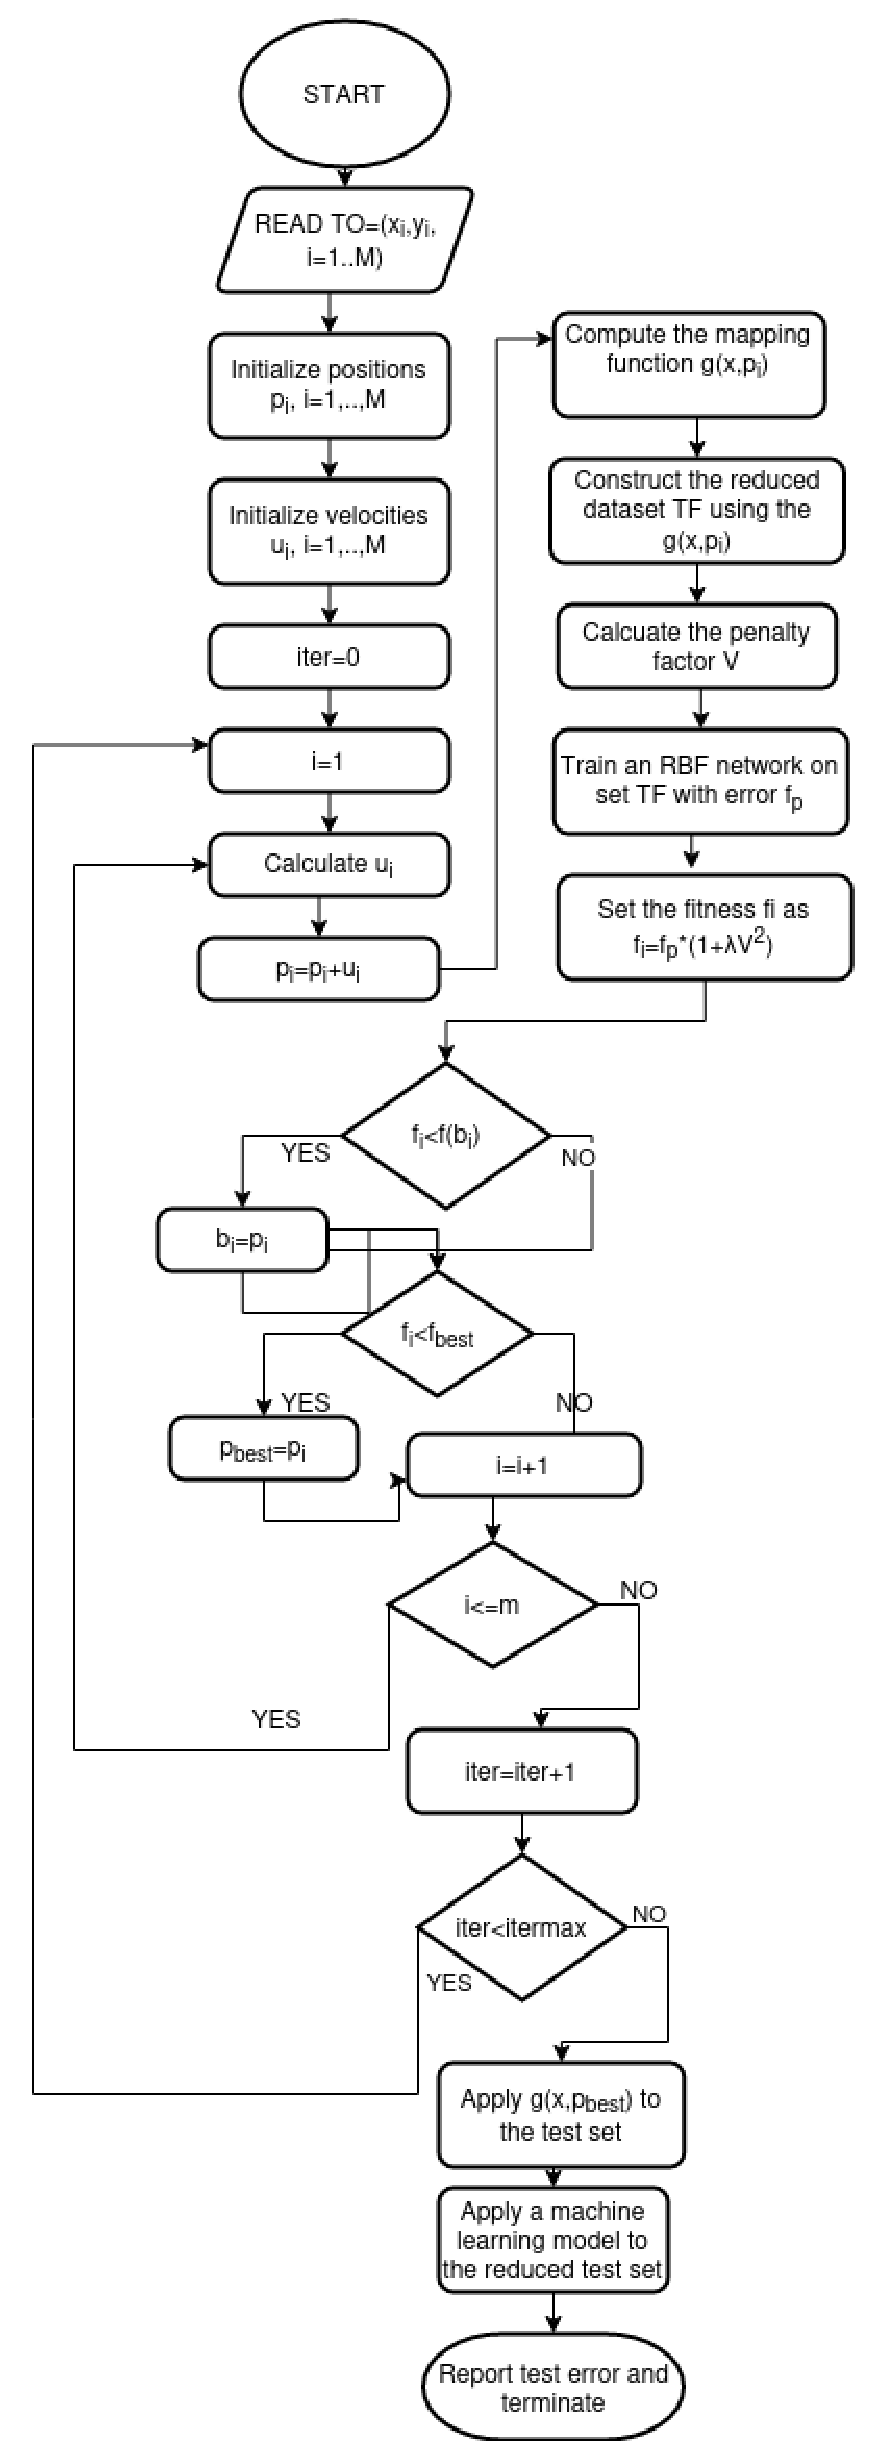
\includegraphics[scale=0.62]{diagram}

\caption{The flowchart for the proposed method.\label{fig:flow}}

\end{figure}


\section{Experiments \label{sec:Experiments}}

The ability of the proposed technique to produce effective artificial
features for class prediction and feature learning will be measured
in this section on a some datasets from the relevant literature. These
problems have been studied by various researchers in the relevant
literature and cover a wide range of research areas from Physics to
Economics. These datasets comes from the relevant websites:
\begin{enumerate}
\item CI dataset repository, \url{https://archive.ics.uci.edu/ml/index.php}
\item Keel repository, \url{https://sci2s.ugr.es/keel/datasets.php}\citep{Keel}.
\item The Stat lib URL \url{ftp://lib.stat.cmu.edu/datasets/index.html }. 
\end{enumerate}
The proposed technique will be compared with a series of known machine
learning techniques and the experimental results are then presented
in the relevant tables.

\subsection{Experimental datasets }

The classification problems used in the experiments have as follows:
\begin{enumerate}
\item \textbf{Appendicitis}, a medical dataset \citep{appendicitis,appendicitis2}. 
\item \textbf{Australian} dataset \citep{australian}, an dataset concerning
economical transactions in banks.
\item \textbf{Balance} dataset, a dataset generated to model psychological
experimental results\citep{balance}.
\item \textbf{Bands} dataset, a dataset used in rotogravure printing \citep{bands}.
\item \textbf{Dermatology} dataset \citep{dermatology}, a medical dataset
used to detect the type of Eryhemato-Squamous Disease. 
\item \textbf{Hayes Roth} dataset \citep{hayesroth}.
\item \textbf{Heart} dataset \citep{heart}, a medical dataset used to detect
heart diseases. 
\item \textbf{House Votes} dataset \citep{housevotes}, a dataset related
to the Congressional voting records of USA.
\item \textbf{Ionosphere} dataset, used to classify measurements from the
ionosphere and it has been examined in a variety of research papers
\citep{ion1,ion2}.
\item \textbf{Liver disorder} dataset \citep{liver1,liver2}, a dataset
used for medical purposes.
\item \textbf{Mammography} dataset \citep{mammographic}, a medical dataset
used for breast cancer diagnosis.
\item \textbf{Parkinson's} dataset \citep{parkinsons1,parkinsons2}, a dataset
used to detect the Parkinson's decease using voice measurements.
\item \textbf{Puma} dataset \citep{pima}, a dataset used for medical purposes.
\item \textbf{Pop failures} dataset \citep{popfailures}, a dataset related
to meteorological data.
\item \textbf{Regions2} dataset, a medical dataset for liver biopsy images
\citep{regions}. 
\item \textbf{Suharto} dataset \citep{saheart}, a medical dataset. 
\item \textbf{Segment} dataset \citep{segment}, a dataset related to image
segmentation.
\item \textbf{BC} dataset \citep{wdbc} used in breast tumors. 
\item \textbf{Wine} dataset, a dataset related to chemical analysis of wines
\citep{wine1,wine2}.
\item \textbf{EEG} datasets \citep{eeg1,eeg2}, it is an EEG dataset and
the following cases were used in the experiments: 
\begin{enumerate}
\item Z\_F\_S, 
\item ZOE\_NF\_S
\item ZONE\_S.
\end{enumerate}
\item \textbf{Zoo} dataset \citep{zoo}.
\end{enumerate}
The regression datasets used in the relevant experiments have as follows:
\begin{enumerate}
\item \textbf{Abalone} dataset \citep{abalone}, a dataset used to predict
the age of abalones.
\item \textbf{Airfoil }dataset, a dataset provided by NASA \citep{airfoil}
obtained from a series of aerodynamic and acoustic tests.
\item \textbf{Baseball} dataset, a dataset related to the salary of baseball
players.
\item \textbf{BK} dataset \citep{Stat}, a dataset that was used to calculate
the points in a basketball game. 
\item \textbf{BL} dataset, used in machine problems.
\item \textbf{Concrete} dataset \citep{concrete}, a civil engineering dataset
to calculate The concrete compressive strength
\item \textbf{Dee} dataset, used to estimate the daily average price of
KWh electricity energy in Spain.
\item \textbf{Diabetes} dataset, a medical dataset.
\item \textbf{Housing} dataset \citep{key23}.
\item \textbf{FA} dataset, used to fit body fat to other measurements. 
\item \textbf{MB} dataset \citep{key21}. 
\item \textbf{MORTGAGE} dataset, holding economic data from USA. The goal
is to predict the 30-Year Conventional Mortgage Rate. 
\item \textbf{PU }dataset, (Pyrimidines problem)\citep{pydataset}.
\item \textbf{Quake} dataset, used to approximate the strength of a earthquake
given its the depth of its focal point, its latitude and its longitude. 
\item \textbf{Treasure} dataset, which contains Economic data information
of USA, where the the goal is to predict 1-Month CD Rate. 
\end{enumerate}

\subsection{Experimental results}

In order to give greater credibility to the experiments carried out,
the method of 10 - fold cross validation was incorporated for every
experimental dataset. Every experiment was repeated 30 times using
different seeds for the random generator each time. All the used code
was implemented in ANSI C++ using the OPTIMUMS programming library
for optimization purposes, freely available from \url{https://github.com/itsoulos/OPTIMUMS/}.
For the classification datasets, the average classification error
as measured in the test set is reported, while for the regression
datasets the average regression error is reported. Here, by the term
classification error, we mean the percentage of patterns in the test
set that are classified into a different class than expected. Also,
in every table, an additional column denoted as AVERAGE is added to
show the average classification or regression error for the corresponding
datasets. The values for the experimental parameters are shown in
Table \ref{tab:values}.

\begin{table}[H]

\caption{The values for every parameter used in the experiments.\label{tab:values}}

\centering{}%
\begin{tabular}{|c|c|c|}
\hline 
PARAMETER & MEANING & VALUE\tabularnewline
\hline 
\hline 
$m$ & Particles or Chromosomes & 200\tabularnewline
\hline 
$H$ & Number of hidden nodes  & 10\tabularnewline
\hline 
$\mbox{iter}_{\mbox{max}}$ & Maximum number of iterations & 200\tabularnewline
\hline 
$L_{\mbox{max}}$ & Limit used in penalty calculation & 100\tabularnewline
\hline 
$\lambda$ & Penalty factor & 100\tabularnewline
\hline 
\end{tabular}
\end{table}
In all techniques the same parameter sets and the same random numbers
have been used in order to have a fair comparison of the experimental
results.

In the first phase the proposed technique will generate new artificial
features from the existing ones with the help of a technique guided
by the partnership of Particle Swarm Optimization and Grammatical
Evolution. In the second phase of the technique, these features will
be used to modify the original test set to which any machine learning
method can now be applied. In the second phase of the current work,
two different techniques will be used: an RF neural network and an
artificial neural network which will be trained using a genetic algorithm.
This is done in order to establish the potential of the proposed procedure
to improve the performance of both simple machine learning models
and complex models. The proposed technique that created artificial
features is compared on the same datasets against a series of well
- known method from the relevant literature: 
\begin{enumerate}
\item A genetic algorithm with $m$ chromosomes, denotes as GENETIC in the
experimental tables. This genetic algorithm is used to train an artificial
neural network with $H$ hidden nodes. After the termination of the
genetic algorithm the local optimization method BEFOGS is applied
to the best chromosome of the population.
\item The Radial Basis Function (RF) network \citep{rbf1} with $H$ processing
nodes.
\item The optimization method Adam \citep{Adam}, used to train an artificial
neural network with $H$ hidden nodes.
\item The Prop optimization method \citep{rpropnn1,rpropnn2}, used to train
an artificial neural network with $H$ hidden nodes.
\item The NEAT method (Revolution of Augmenting Typologies ) \citep{neat}.
\end{enumerate}
The experimental results using the above methods on the classification
datasets are shown in Table \ref{tab:exp1} and the results for the
regression datasets are illustrated in Table \ref{tab:exp2}.

\begin{table}[H]
\caption{Average classification error for the classification datasets using
the well - known methods. \label{tab:exp1}}

\centering{}%
\begin{tabular}{|c|c|c|c|c|c|}
\hline 
DATASET & GENETIC & RF & ADAM & PROP & NEAT\tabularnewline
\hline 
\hline 
Appendicitis & 18.10\% & 12.23\% & 16.50\% & 16.30\% & 17.20\%\tabularnewline
\hline 
Australian & 32.21\% & 34.89\% & 35.65\% & 36.12\% & 31.98\%\tabularnewline
\hline 
Balance & 8.97\% & 33.42\% & 7.87\% & 8.81\% & 23.14\%\tabularnewline
\hline 
Bands & 35.75\% & 37.22\% & 36.25\% & 36.32\% & 34.30\%\tabularnewline
\hline 
Dermatology & 30.58\% & 62.34\% & 26.14\% & 15.12\% & 32.43\%\tabularnewline
\hline 
Hayes Roth & 56.18\% & 64.36\% & 59.70\% & 37.46\% & 50.15\%\tabularnewline
\hline 
Heart & 28.34\% & 31.20\% & 38.53\% & 30.51\% & 39.27\%\tabularnewline
\hline 
House Votes & 6.62\% & 6.13\% & 7.48\% & 6.04\% & 10.89\%\tabularnewline
\hline 
Ionosphere & 15.14\% & 16.22\% & 16.64\% & 13.65\% & 19.67\%\tabularnewline
\hline 
Liver disorder & 31.11\% & 30.84\% & 41.53\% & 40.26\% & 30.67\%\tabularnewline
\hline 
Lymography & 23.26\% & 25.31\% & 29.26\% & 24.67\% & 33.70\%\tabularnewline
\hline 
Mammography & 19.88\% & 21.38\% & 46.25\% & 18.46\% & 22.85\%\tabularnewline
\hline 
Parkinson's & 18.05\% & 17.42\% & 24.06\% & 22.28\% & 18.56\%\tabularnewline
\hline 
Puma & 32.19\% & 25.78\% & 34.85\% & 34.27\% & 34.51\%\tabularnewline
\hline 
Pop failures & 5.94\% & 7.04\% & 5.18\% & 4.81\% & 7.05\%\tabularnewline
\hline 
Regions2 & 29.39\% & 38.29\% & 29.85\% & 27.53\% & 33.23\%\tabularnewline
\hline 
Suharto & 34.86\% & 32.19\% & 34.04\% & 34.90\% & 34.51\%\tabularnewline
\hline 
Segment & 57.72\% & 59.68\% & 49.75\% & 52.14\% & 66.72\%\tabularnewline
\hline 
BC & 8.56\% & 7.27\% & 35.35\% & 21.57\% & 12.88\%\tabularnewline
\hline 
Wine & 19.20\% & 31.41\% & 29.40\% & 30.73\% & 25.43\%\tabularnewline
\hline 
Z\_F\_S & 10.73\% & 13.16\% & 47.81\% & 29.28\% & 38.41\%\tabularnewline
\hline 
ZOE\_NF\_S & 8.41\% & 9.02\% & 47.43\% & 6.43\% & 43.75\%\tabularnewline
\hline 
ZONE\_S & 2.60\% & 4.03\% & 11.99\% & 27.27\% & 5.44\%\tabularnewline
\hline 
ZOO & 16.67\% & 21.93\% & 14.13\% & 15.47\% & 20.27\%\tabularnewline
\hline 
\textbf{AVERAGE} & \textbf{22.94\%} & \textbf{26.78\%} & \textbf{30.24\%} & \textbf{24.60\%} & \textbf{28.63\%}\tabularnewline
\hline 
\end{tabular}
\end{table}

\begin{table}[H]
\caption{Average regression error using the well - known methods for the regression
datasets.\label{tab:exp2}}

\centering{}%
\begin{tabular}{|c|c|c|c|c|c|}
\hline 
DATASET & GENETIC & RF & ADAM & PROP & NEAT\tabularnewline
\hline 
\hline 
ABALONE & 7.17 & 7.37 & 4.30 & 4.55 & 9.88\tabularnewline
\hline 
AIRFOIL & 0.003 & 0.27 & 0.005 & 0.002 & 0.067\tabularnewline
\hline 
BASEBALL & 103.60 & 93.02 & 77.90 & 92.05 & 100.39\tabularnewline
\hline 
BK & 0.027 & 0.02 & 0.03 & 1.599 & 0.15\tabularnewline
\hline 
BL & 5.74 & 0.01 & 0.28 & 4.38 & 0.05\tabularnewline
\hline 
CONCRETE & 0.0099 & 0.011 & 0.078 & 0.0086 & 0.081\tabularnewline
\hline 
DEE & 1.013 & 0.17 & 0.63 & 0.608 & 1.512\tabularnewline
\hline 
DIABETES & 19.86 & 0.49 & 3.03 & 1.11 & 4.25\tabularnewline
\hline 
HOUSING & 43.26 & 57.68 & 80.20 & 74.38 & 56.49\tabularnewline
\hline 
FA & 1.95 & 0.02 & 0.11 & 0.14 & 0.19\tabularnewline
\hline 
MB & 3.39 & 2.16 & 0.06 & 0.055 & 0.061\tabularnewline
\hline 
MORTGAGE & 2.41 & 1.45 & 9.24 & 9.19 & 14.11\tabularnewline
\hline 
PU & 1.21 & 0.02 & 0.09 & 0.039 & 0.075\tabularnewline
\hline 
QUAKE & 0.04 & 0.071 & 0.06 & 0.041 & 0.298\tabularnewline
\hline 
TREASURY & 2.929 & 2.02 & 11.16 & 10.88 & 15.52\tabularnewline
\hline 
\textbf{AVERAGE} & \textbf{12.84} & \textbf{10.30} & \textbf{11.70} & \textbf{12.44} & \textbf{12.70}\tabularnewline
\hline 
\end{tabular}
\end{table}
The results using the proposed method and for the construction of
2,3 and 4 artificial features are presented in the relevant tables,
\ref{tab:tabClass} and \ref{tab:tabRegression}. The RF column represents
the experimental results in which, after the construction of the artificial
features, a RF network with $H$ processing nodes is applied on the
modified dataset. Also, the column GENETIC in tables \ref{tab:tabClass},
\ref{tab:tabRegression} stands for the results obtained by the application
of a genetic algorithm with $m$ chromosomes to the modified dataset,
when the feature creation procedure has been finished.

\begin{table}[H]
\caption{Experimental results for the classification datasets using the proposed
method. Number in cells denote average classification error as measured
on the test set.\label{tab:tabClass}. The variable $f$ corresponds
to the number of artificial features created by the proposed method.}

\centering{}%
\begin{tabular}{|c|c|c|c|c|c|c|}
\hline 
 & \multicolumn{2}{c|}{$f=2$} & \multicolumn{2}{c|}{$f=3$} & \multicolumn{2}{c|}{$f=4$}\tabularnewline
\hline 
\hline 
DATASET & RF & GENETIC & RF & GENETIC & RF & GENETIC\tabularnewline
\hline 
APPENDICITIS & 15.40\% & 14.33\% & 16.90\% & 15.77\% & 15.97\% & 17.30\%\tabularnewline
\hline 
AUSTRALIAN & 15.49\% & 14.48\% & 14.53\% & 15.33\% & 14.75\% & 15.97\%\tabularnewline
\hline 
BALANCE & 16.67\% & 2.89\% & 22.54\% & 4.94\% & 17.26\% & 4.62\%\tabularnewline
\hline 
BANDS & 38.09\% & 38.13\% & 37.09\% & 39.22\% & 37.22\% & 35.51\%\tabularnewline
\hline 
DERMATOLOGY & 41.58\% & 30.37\% & 35.46\% & 25.44\% & 40.45\% & 21.97\%\tabularnewline
\hline 
HAYES ROTH & 37.41\% & 27.92\% & 38.10\% & 25.74\% & 39.59\% & 25.82\%\tabularnewline
\hline 
HEART & 21.53\% & 17.13\% & 17.64\% & 16.87\% & 19.63\% & 15.69\%\tabularnewline
\hline 
HOUSE VOTES & 6.36\% & 3.78\% & 7.17\% & 3.25\% & 4.25\% & 3.52\%\tabularnewline
\hline 
IONOSPHERE & 10.32\% & 10.17\% & 10.12\% & 10.01\% & 11.42\% & 9.02\%\tabularnewline
\hline 
LIVERDISORDER & 34.23\% & 32.33\% & 35.84\% & 32.97\% & 35.93\% & 30.74\%\tabularnewline
\hline 
LYMOGRAPHY & 34.93\% & 28.67\% & 32.00\% & 23.00\% & 29.00\% & 23.83\%\tabularnewline
\hline 
MAMMOGRAPHIC & 16.92\% & 16.51\% & 16.47\% & 16.35\% & 17.54\% & 16.50\%\tabularnewline
\hline 
PARKINSONS & 11.14\% & 13.00\% & 11.30\% & 11.11\% & 12.95\% & 9.42\%\tabularnewline
\hline 
PIMA & 22.85\% & 22.76\% & 24.93\% & 24.67\% & 24.25\% & 24.20\%\tabularnewline
\hline 
POPFAILURES & 7.32\% & 7.41\% & 6.96\% & 7.62\% & 5.96\% & 5.67\%\tabularnewline
\hline 
REGIONS2 & 28.52\% & 26.84\% & 24.91\% & 25.28\% & 25.35\% & 24.93\%\tabularnewline
\hline 
SAHEART & 29.29\% & 28.63\% & 28.92\% & 30.31\% & 28.25\% & 30.25\%\tabularnewline
\hline 
SEGMENT & 52.69\% & 45.59\% & 46.83\% & 41.06\% & 50.15\% & 39.52\%\tabularnewline
\hline 
WDBC & 5.00\% & 4.66\% & 5.76\% & 4.97\% & 5.13\% & 3.84\%\tabularnewline
\hline 
WINE & 8.92\% & 7.22\% & 6.76\% & 5.75\% & 6.00\% & 5.86\%\tabularnewline
\hline 
Z\_F\_S & 7.91\% & 8.37\% & 7.89\% & 7.67\% & 5.21\% & 6.86\%\tabularnewline
\hline 
ZOE\_NF\_S & 6.90\% & 6.85\% & 6.95\% & 5.65\% & 6.24\% & 5.28\%\tabularnewline
\hline 
ZONE\_S & 3.08\% & 3.40\% & 2.44\% & 2.52\% & 3.47\% & 3.33\%\tabularnewline
\hline 
ZOO & 26.47\% & 7.83\% & 31.73\% & 10.03\% & 28.70\% & 11.57\%\tabularnewline
\hline 
\textbf{AVERAGE} & \textbf{20.79\%} & \textbf{17.47\%} & \textbf{20.39\%} & \textbf{16.90\%} & \textbf{20.19\%} & \textbf{16.30\%}\tabularnewline
\hline 
\end{tabular}
\end{table}
\begin{table}[H]
\caption{Experimental results on the regression datasets using the proposed
method. The number in cells denote average regression error as measured
on the test set.\label{tab:tabRegression}The variable $f$ corresponds
to the number of artificial features created by the proposed method.}

\centering{}%
\begin{tabular}{|c|c|c|c|c|c|c|}
\hline 
 & \multicolumn{2}{c|}{$f=2$} & \multicolumn{2}{c|}{$f=3$} & \multicolumn{2}{c|}{$f=4$}\tabularnewline
\hline 
\hline 
DATASET & RF & GENETIC & RF & GENETIC & RF & GENETIC\tabularnewline
\hline 
ABALONE & 4.361 & 3.518 & 4.159 & 3.839 & 4.859 & 3.786\tabularnewline
\hline 
AIRFOIL & 0.003 & 0.001 & 0.003 & 0.001 & 0.003 & 0.001\tabularnewline
\hline 
BASEBALL & 66.00 & 53.74 & 60.79 & 57.04 & 66.19 & 61.69\tabularnewline
\hline 
BK & 0.022 & 0.031 & 0.021 & 0.029 & 0.019 & 0.023\tabularnewline
\hline 
BL & 0.413 & 0.0001 & 0.019 & 0.007 & 0.043 & 0.011\tabularnewline
\hline 
CONCRETE & 0.008 & 0.006 & 0.007 & 0.005 & 0.008 & 0.004\tabularnewline
\hline 
DEE & 0.259 & 0.252 & 0.339 & 0.286 & 0.609 & 0.5\tabularnewline
\hline 
DIABETES & 0.611 & 0.832 & 0.634 & 1.411 & 0.857 & 1.157\tabularnewline
\hline 
HOUSING & 22.387 & 15.583 & 18.614 & 13.602 & 14.83 & 13.208\tabularnewline
\hline 
FA & 0.056 & 0.011 & 0.015 & 0.011 & 0.015 & 0.012\tabularnewline
\hline 
MB & 0.258 & 0.087 & 0.115 & 0.078 & 0.342 & 0.072\tabularnewline
\hline 
MORTGAGE & 0.621 & 0.046 & 0.65 & 0.037 & 0.078 & 0.04\tabularnewline
\hline 
PU & 2.894 & 0.14 & 0.936 & 0.029 & 0.724 & 0.031\tabularnewline
\hline 
QUAKE & 0.069 & 0.036 & 0.057 & 0.037 & 0.04 & 0.037\tabularnewline
\hline 
TREASURY & 0.912 & 0.088 & 0.874 & 0.084 & 0.173 & 0.076\tabularnewline
\hline 
\textbf{AVERAGE} & \textbf{6.59} & \textbf{4.96} & \textbf{5.82} & \textbf{5.10} & \textbf{5.92} & \textbf{5.38}\tabularnewline
\hline 
\end{tabular}
\end{table}

The experimental results are of great interest, as one can see from
their careful study, the proposed technique is able to significantly
reduce the error in the corresponding test sets. Especially in the
case of regression problems, the reduction in error is on average
greater than 50\%. Moreover, the usage of a neural network trained
by a genetic algorithm on the modified datasets, gives clearly better
results than the use of an RF neural network, especially in the classification
datasets. An additional test was performed for the regression datasets,
where the number of particles in PESO algorithm increases from 100
to 400 and the results are graphically illustrated in Figure \ref{fig:psodiagram}.

\begin{figure}[H]
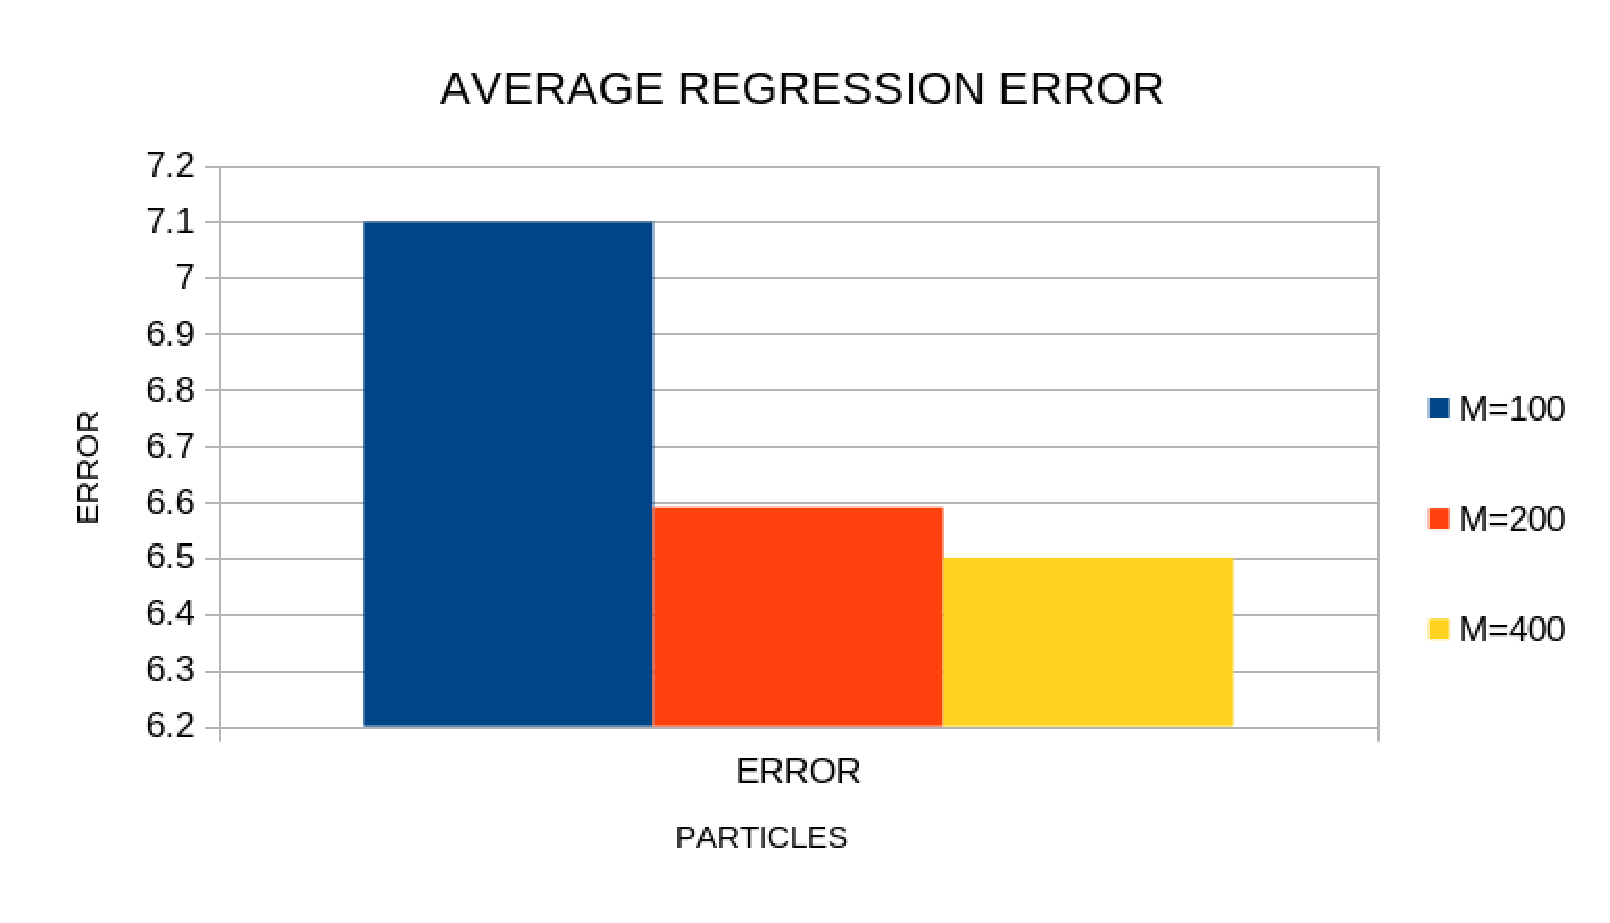
\includegraphics[scale=0.5]{pso_diagram}

\caption{Average regression error for all regression datasets using the proposed
method. The number of PESO particles increases from 100 to 400 and
the number of constructed features was set to $f=2$.\label{fig:psodiagram}}

\end{figure}
 Judging from the results, we can observe that the selection of 200
particles in the experimental results was an optimal choice and a
compromise between the speed and efficiency of the method, as adding
another 200 particles to the Particle Swarm Optimization did not significantly
improve the efficiency of the proposed method.

Moreover, a graphical comparison between the genetic algorithm when
applied to artificial datasets and the genetic algorithm when applied
to the original classification datasets is given in Figure \ref{fig:geneticComparison}.
The same graphical comparison is also shown for the RF model in Figure
\ref{fig:comparisonRbf}. And in these figures, the ability of the
proposed method to drastically reduce learning error through the construction
of artificial features is evident.

\begin{figure}[H]
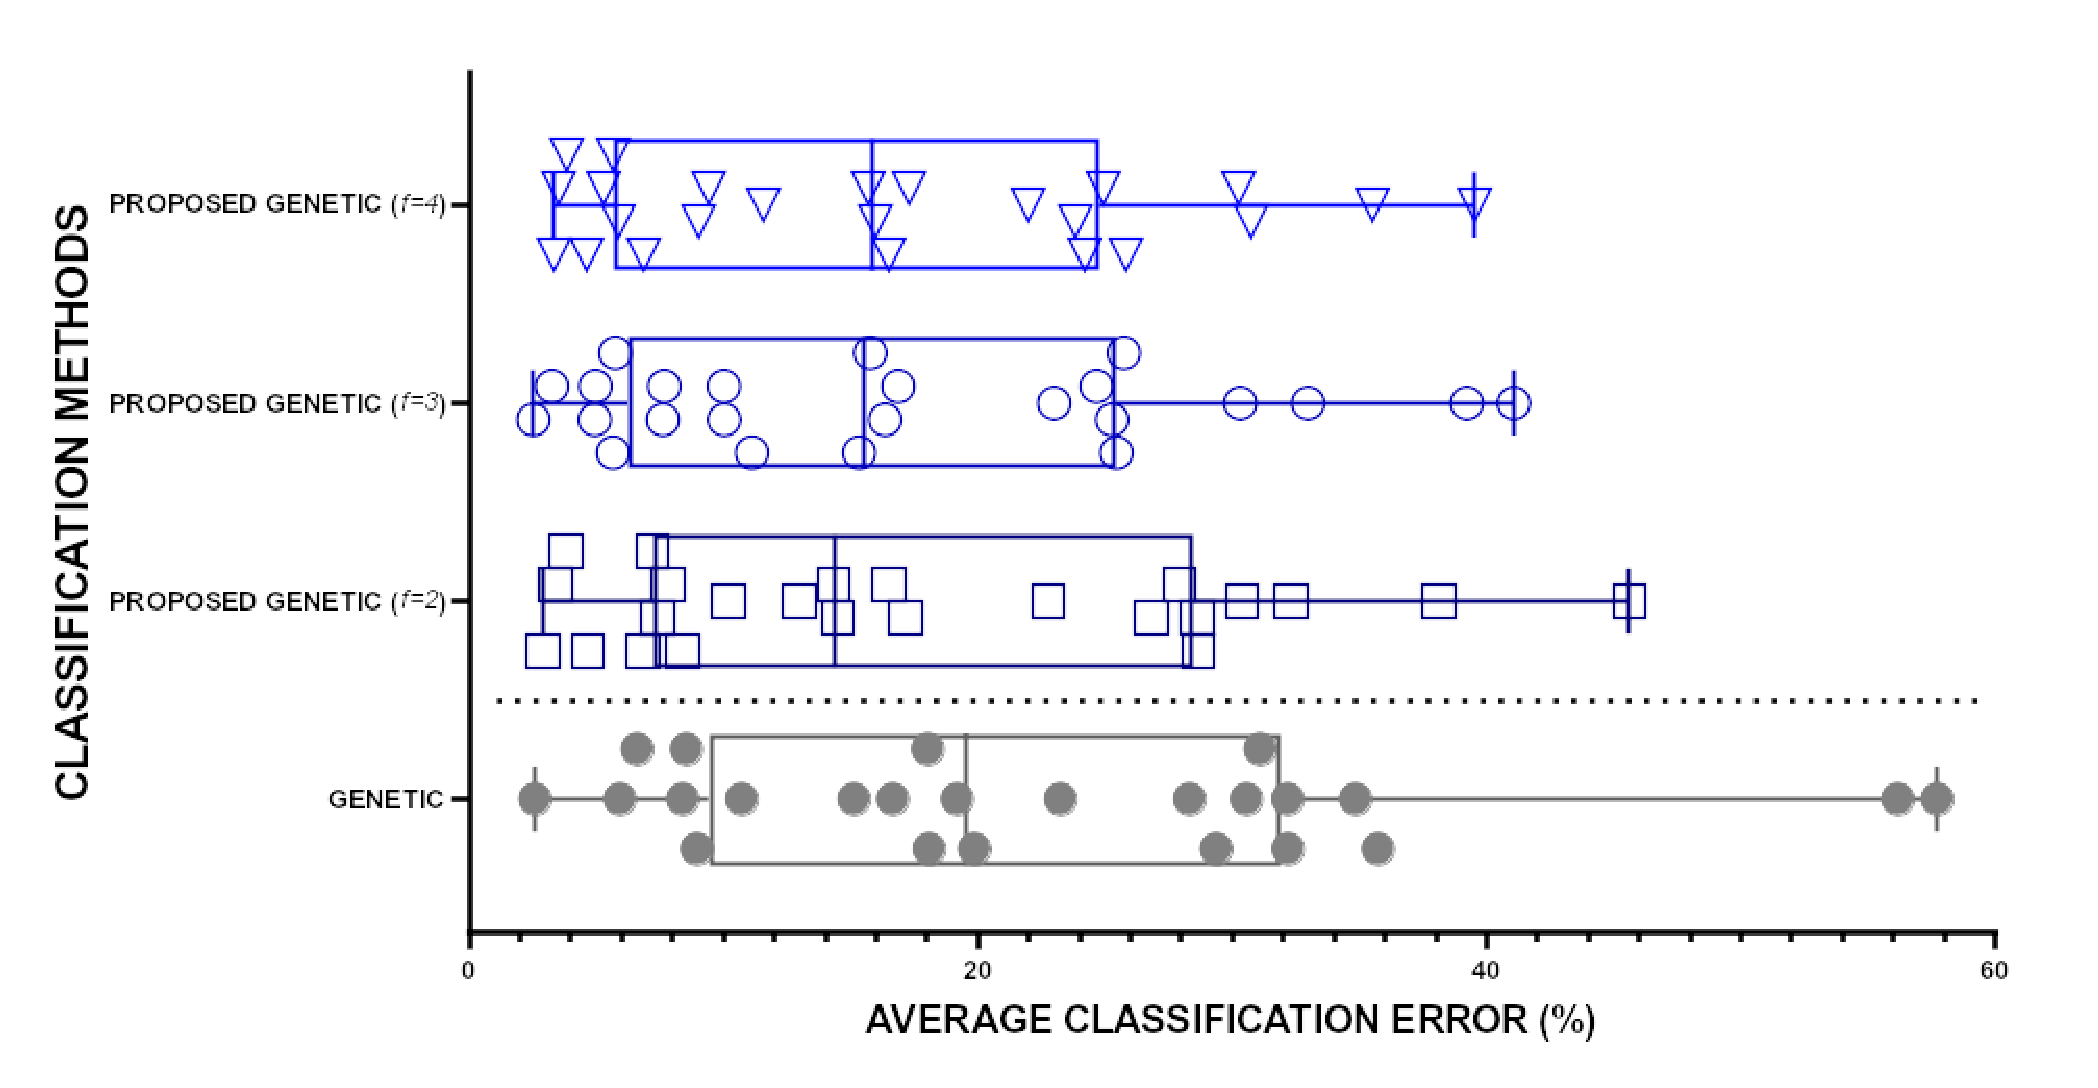
\includegraphics[scale=0.45]{genetic_all}

\caption{Comparison of the proposed Genetic classification algorithm for the
construction of 2,3 and 4 artificial features (blue color) vs. a welkin
Genetic classification algorithm (Grey color) to the 24 different
datasets.\label{fig:geneticComparison}}

\end{figure}

\begin{figure}[H]
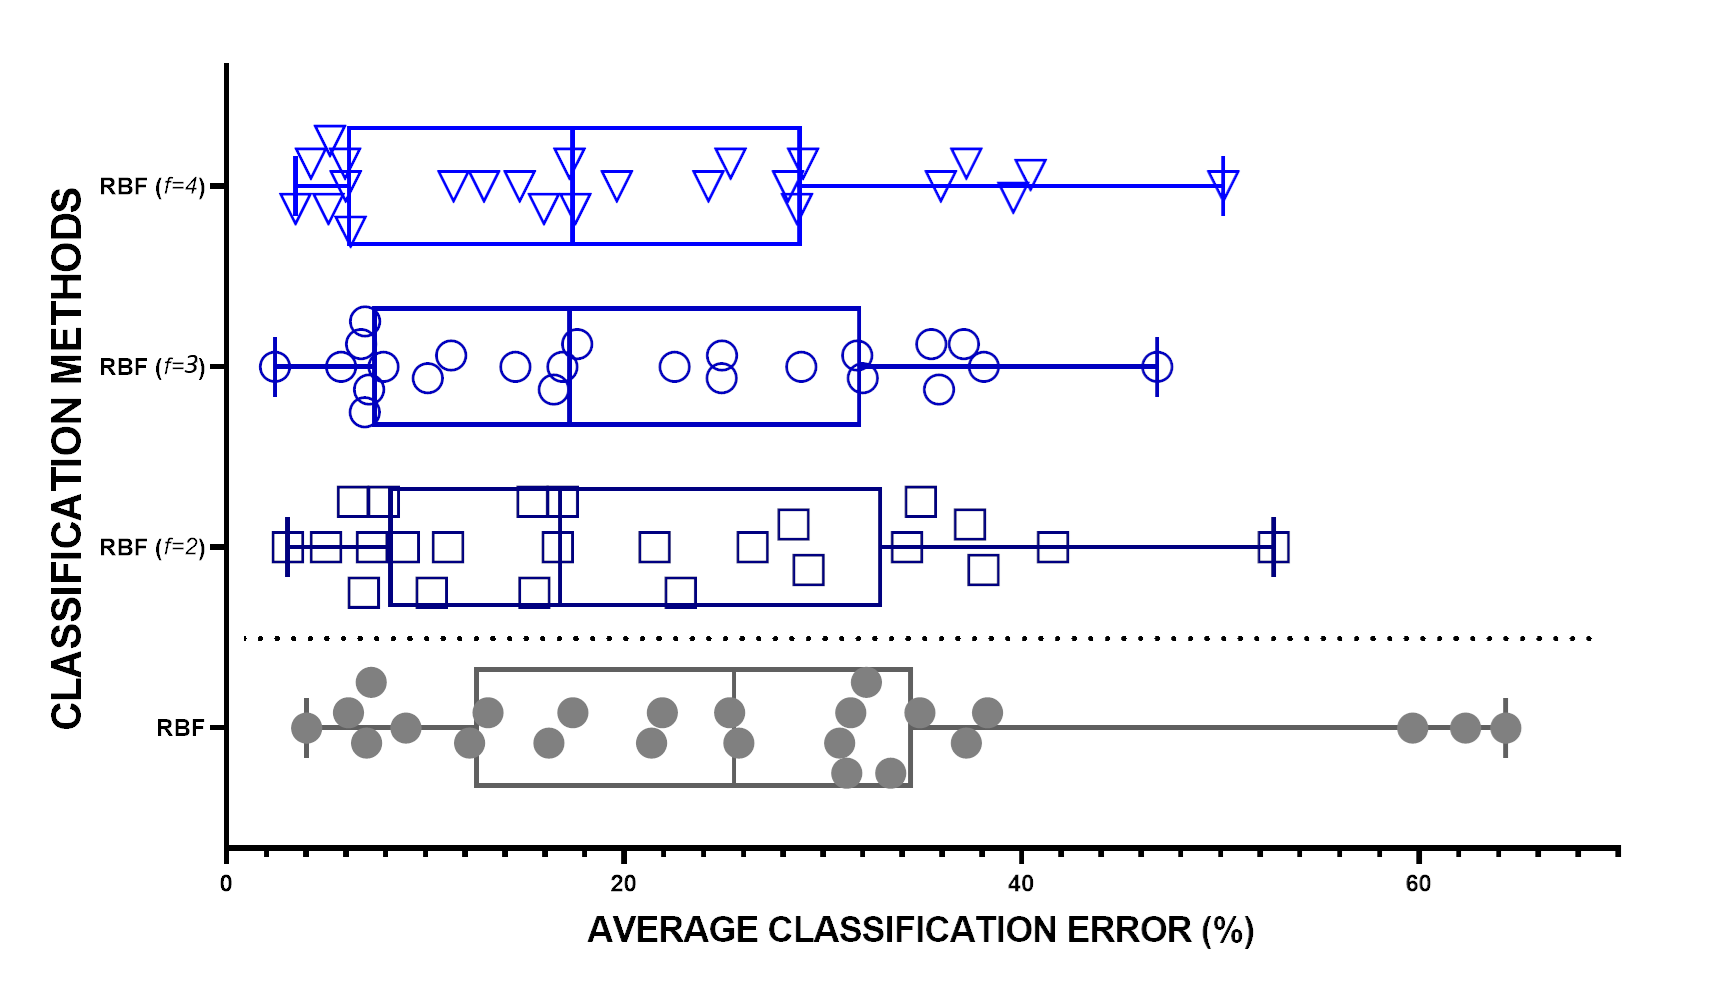
\includegraphics[scale=0.45]{rbf_all}

\caption{Comparison of the proposed RF classification network for the construction
of 2,3 and 4 artificial features (blue color) vs. a welkin RF classification
network (Grey color) to the 24 different datasets.\label{fig:comparisonRbf}}

\end{figure}
Also, in figure \ref{fig:geneticStat} a comparison for the regression
datasets is outlined between the proposed method with the application
of the genetic algorithm in second phase and the genetic algorithm
on the original regression datasets.

\begin{figure}[H]
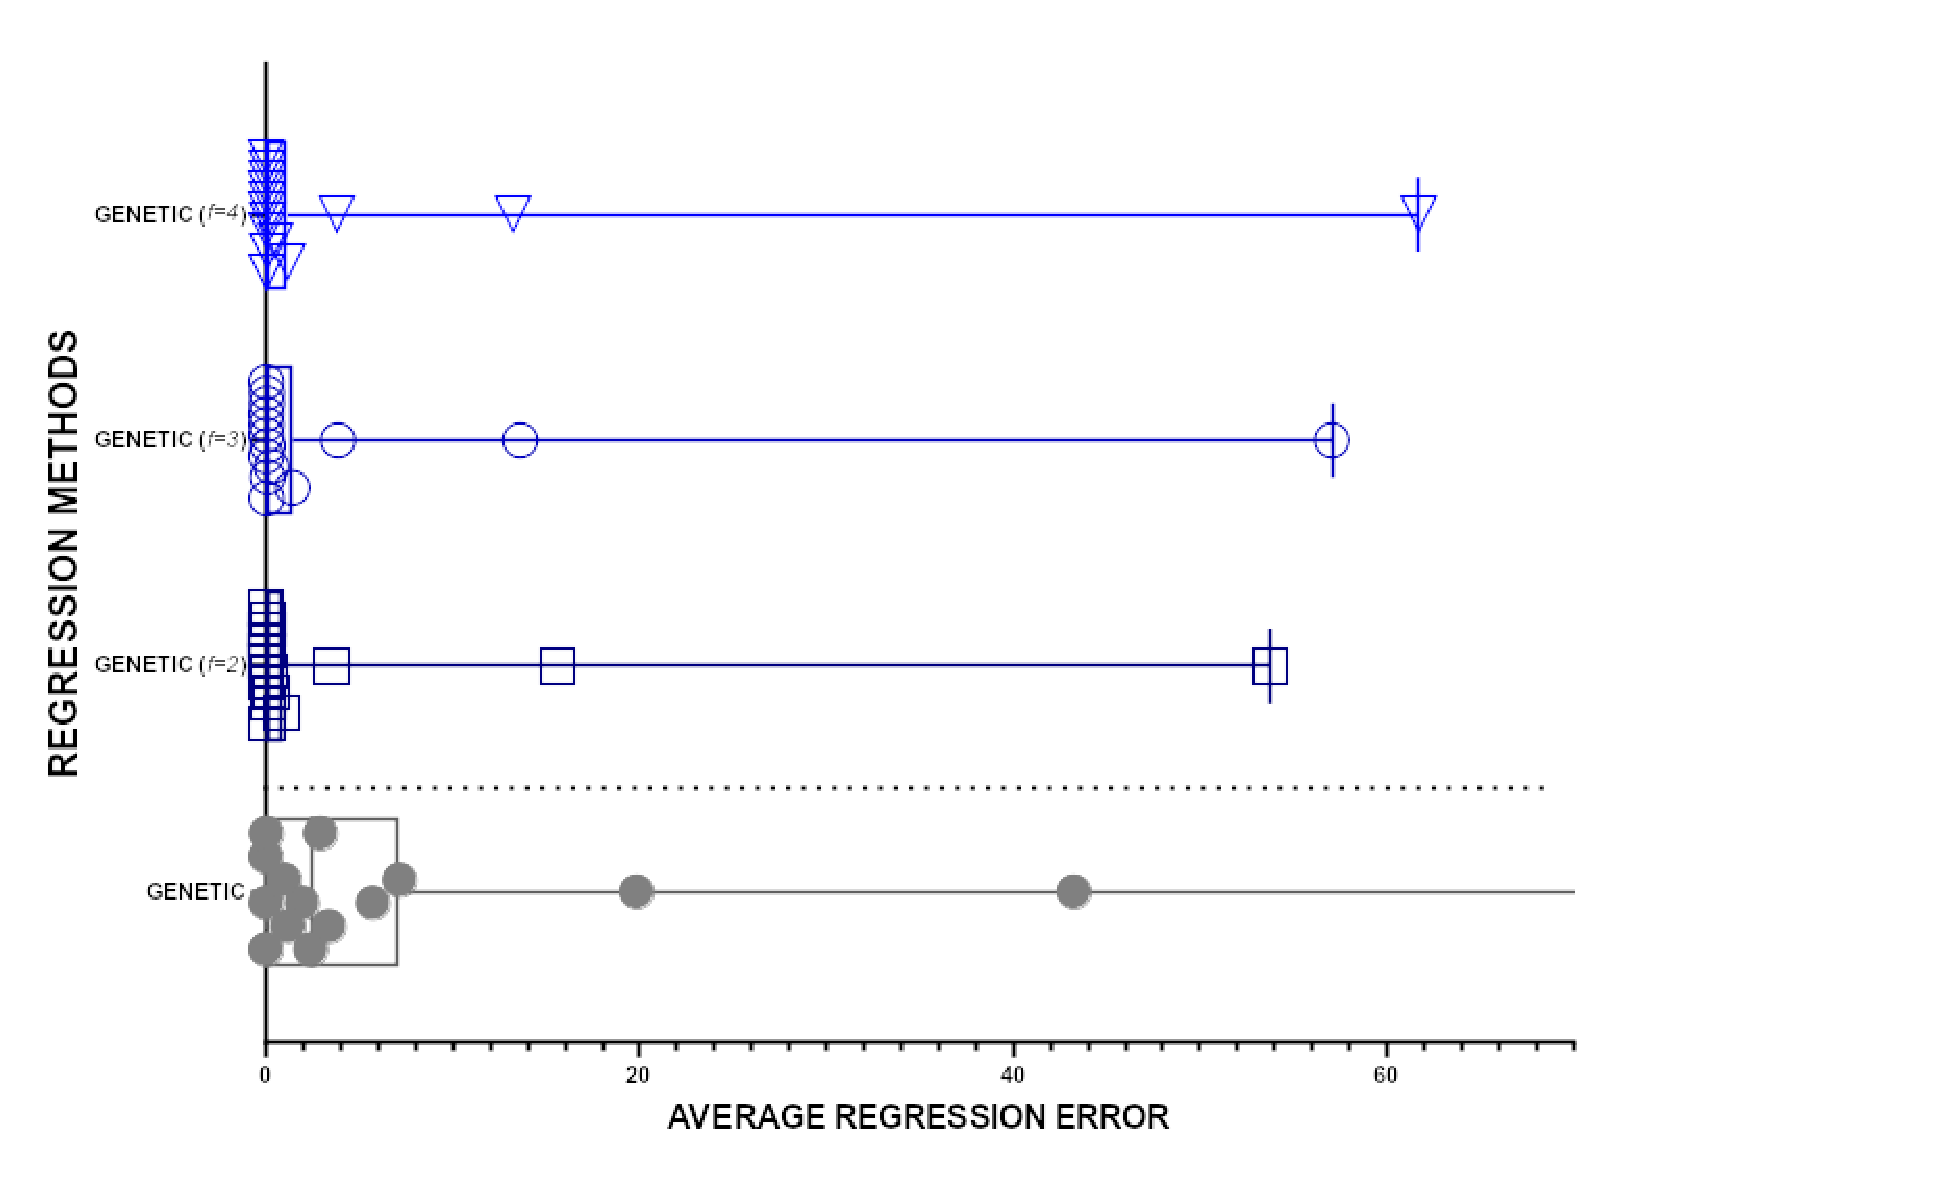
\includegraphics[scale=0.45]{genetic_regression}

\caption{Comparison of the proposed algorithm for the construction of 2,3 and
4 artificial features (blue color) vs. the genetic algorithm (Grey
color) for the regression datasets.\label{fig:geneticStat}}

\end{figure}
Finally, using the Wilcox on sandbank test a comparison is made between
the proposed method and all mentioned machine learning methods for
the classification datasets. This comparison is graphically outlined
in Figure \ref{fig:comparisonAll}.

\begin{figure}[H]
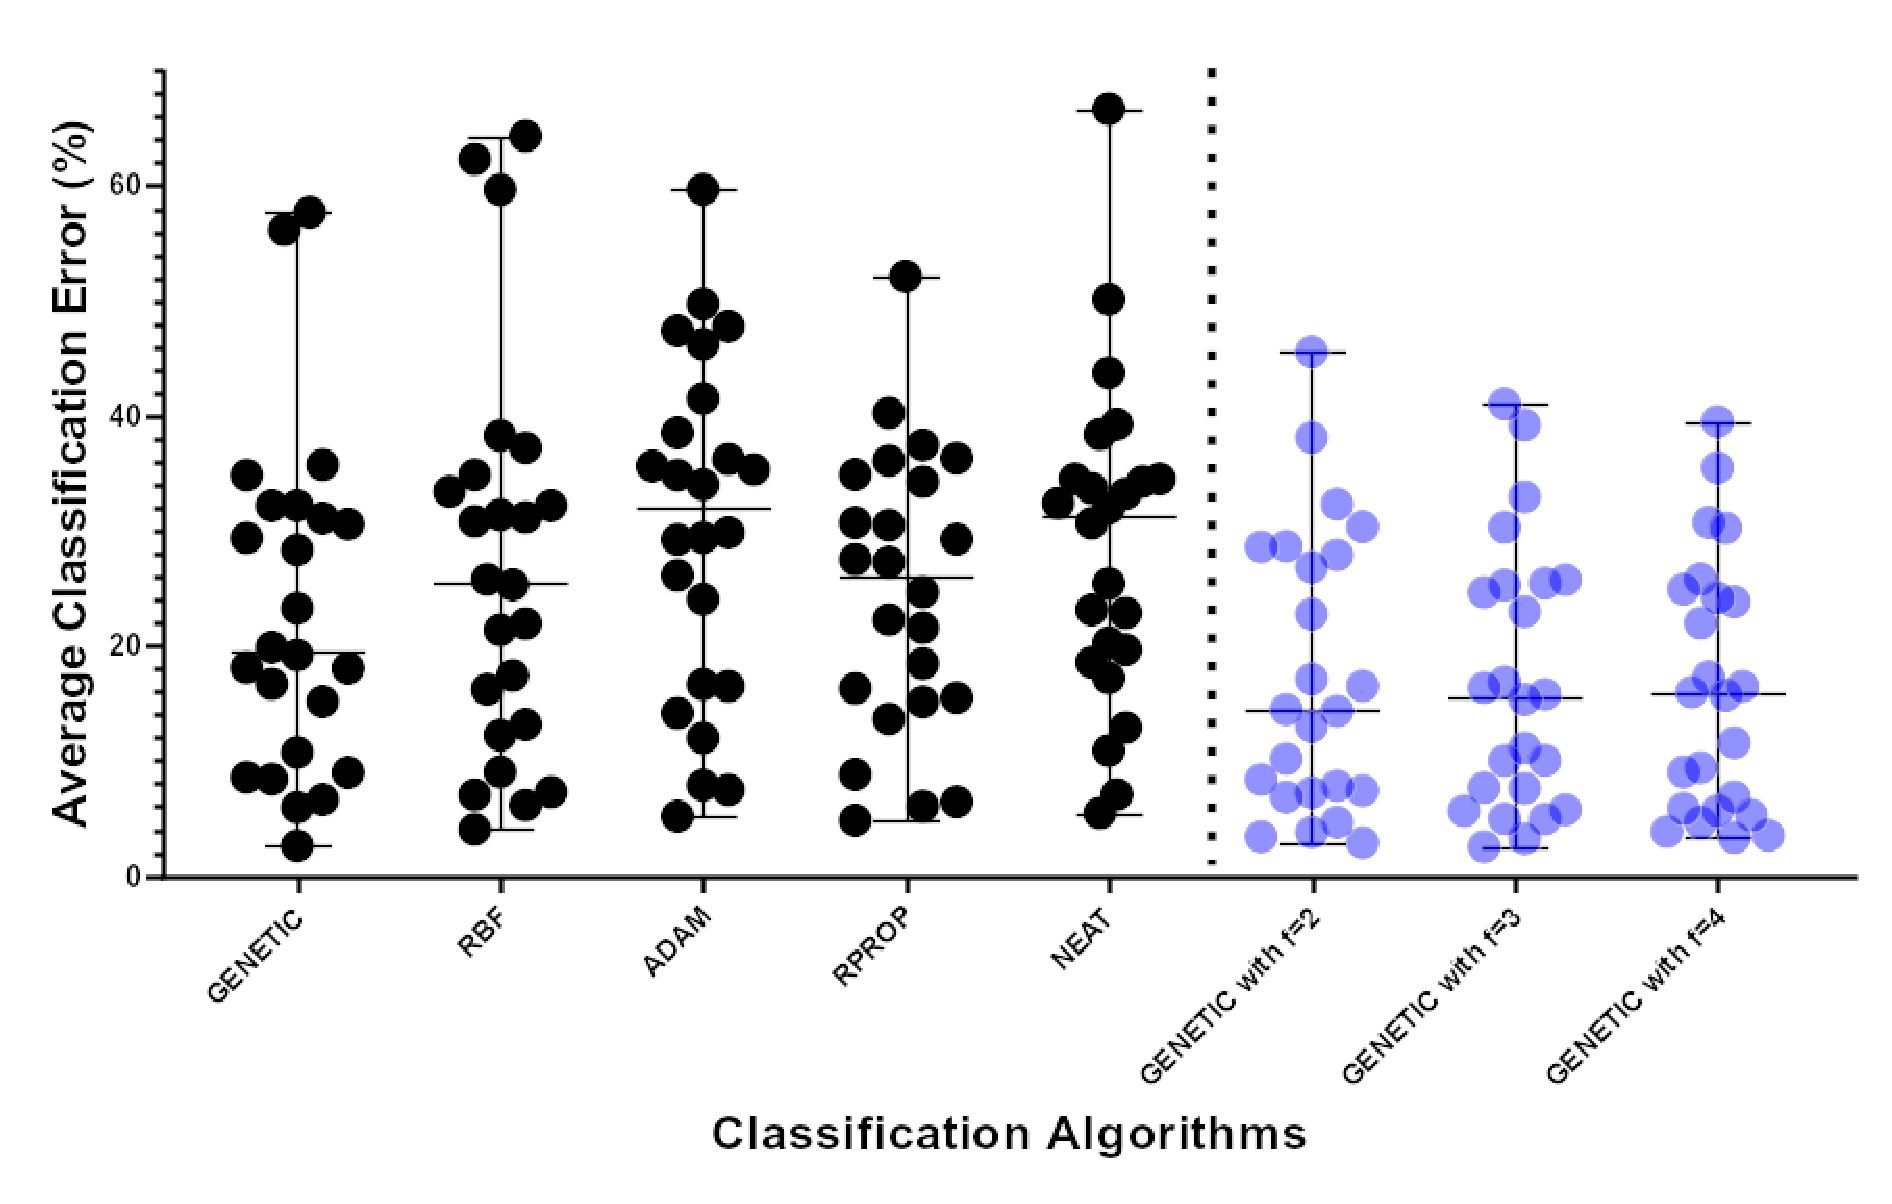
\includegraphics[scale=0.45]{comparison_all}

\caption{The comparison between the proposed method for constructing 2, 3,
and 4 artificial features (blue colour) and several welkin classification
methods (black colour) on 24 different datasets revealed that the
proposed method demonstrated superior performance with statistical
significance. The results were obtained using the Wilcox on sandbank
test. Across all 24 datasets, the proposed method consistently outperformed
the welkin classification methods regarding classification error .\label{fig:comparisonAll}}

\end{figure}
These results suggest that the proposed method has a distinct advantage
over the welkin classification methods when it comes to constructing
artificial features for classification tasks. It offers improved performance
and provides a more effective solution for these datasets

\section{Conclusions\label{sec:Conclusions} }

A hybrid technique that utilizes a Particle Swarm Optimizer and a
feature creation method using Grammatical Evolution was introduced
here. The proposed method can identify possible dependencies between
the original features and can also reduce the number of required features
to a limited number. Also, the method can remove from the set of features
those features that may not contribute to the learning of the data
set by some machine learning model. In addition, to make learning
more efficient, the values of the generated features are bounded within
a value interval using penalty factors. The constructed features are
evaluated in terms of their effectiveness with the help of a fast
machine learning model such as the RF network, even though other more
effective models could also be used. Among the advantages of the proposed
procedure is the fact that it does not require any prior knowledge
of the data set to which it will be applied and furthermore, the procedure
is exactly the same whether it is a data classification problem or
a data fitting problem. The Particle Swarm Optimization method was
used for the production of the characteristics as it has been proven
by the relevant literature to be an extremely efficient technique
and has a limited number of parameters that must be defined by the
user.

The current work was applied on an extended series of widely used
datasets from various fields and was compared against some machine
learning models on the same datasets. From the experimental results,
it was seen that the proposed technique dramatically improves the
performance of traditional learning techniques when applied to artificial
features. The proposed two-stage technique generated artificial features
in the first stage guided by the Particle Swarm Optimization technique,
and in the second stage, either a neural network trained by genetic
algorithm or a RF network was used in the modified test set. In both
cases, the improvement from artificial feature generation in control
error was significant for each learning model.\textbf{ }This improvement
reaches an average of 30\% for data classification and 50\% for data
fitting problems.\textbf{ }In fact, in many cases, the improvement
in test error exceeds 75\%. Moreover, the method appears quite robust,
since increasing the number of particles in the particle swarm optimization
method did not show to significantly reduce the average error in the
test sets. Furthermore, increasing the number of features constructed
does not seem to have a dramatic effect on the performance of the
method, which means that the method is able to achieve good generalization
results even with a limited number of features, which in turn leads
to greatly reducing the number of dimensions of the original problem.
Future work on the method may include the use of parallel techniques
for feature construction to drastically reduce the required execution
time.

\vspace{6pt}


\authorcontributions{I.G.T. and A.T. conceived of the idea and the methodology and I.G.T
has implemented the corresponding software. I.G.T. conducted the experiments,
employing objective functions as test cases, and provided the comparative
experiments. A.T. has performed the necessary statistical tests. All
authors have read and agreed to the published version of the manuscript.}

\funding{This research received no external funding.}

\institutionalreview{Not applicable.}

\informedconsent{Not applicable. }

\institutionalreview{Not applicable.}

\acknowledgments{The experiments of this research work were performed at the high
performance computing system established at Knowledge and Intelligent
Computing Laboratory, Department of Informatics and Telecommunications,
University of Ioannina, acquired with the project “Educational Laboratory
equipment of TEI of Epirus” with MIS 5007094 funded by the Operational
Programme “Epirus” 2014--2020, by ERDF and national funds.}

\conflictsofinterest{The authors declare no conflict of interest.}

\sampleavailability{Not applicable.}

\appendixtitles{}

\appendixstart{}

\appendix

\begin{adjustwidth}{-\extralength}{0cm}{}

\reftitle{References}
\begin{thebibliography}{99}
\bibitem{fc_physics1}E.M. Metodiev, B. Nachman, J. Thaler, Classification
without labels: learning from mixed samples in high energy physics.
J. High Energ. Phys. 2017, article number 174, 2017.

\bibitem{nnphysics1}P. Baldi, K. Cranmer, T. Faucett et al, Parameterized
neural networks for high-energy physics, Eur. Phys. J. C \textbf{76},
2016.

\bibitem{nnphysics2}A. K. Aniyan, K. Thorat, Classifying Radio Galaxies
with the Convolutional Neural Network, The Astrophysical Journal Supplement
Series \textbf{230}, 20, 2017.

\bibitem{nnphysics3}G. Carleo,M. Troyer, Solving the quantum many-body
problem with artificial neural networks, Science \textbf{355}, pp.
602-606, 2017.

\bibitem{fc_chem1}J.N. Wei, D. Duvenaud, A. A. Guzik, Neural Networks
for the Prediction of Organic Chemistry Reactions, ACS Central Science
\textbf{2}, pp. 725-732, 2016.

\bibitem{fc_chem2}C.Qi, A. Fourie, Q. Chen, Neural network and particle
swarm optimization for predicting the unconfined compressive strength
of cemented paste backfill, Construction and Building Materials \textbf{159},
pp. 473-478, 2018.

\bibitem{fc_chem3}H. Gao, T. J. Struble, C.W. Coley, Y. Wang, W.H.
Green, K. F. Jensen, Using Machine Learning To Predict Suitable Conditions
for Organic Reactions, ACS Central Science \textbf{4}, pp. 1465-1476,
2018.

\bibitem{fc_econ1}R. Hafezi, J. Shahrabi, E. Hadavandi, A bat-neural
network multi-agent system (BNNMAS) for stock price prediction: Case
study of DAX stock price, Applied Soft Computing \textbf{29}, pp.
196-210, 2015.

\bibitem{fc_econ2}X. Pang, Y. Zhou, P. Wang et al, An innovative
neural network approach for stock market prediction, J Supercomput
\textbf{76}, pp. 2098--2118, 2020.

\bibitem{fc_pollution1}A. Russo, P.G. Lind, F. Raischel, R. Trigo,
M. Mendes, Neural network forecast of daily pollution concentration
using optimal meteorological data at synoptic and local scales, Atmospheric
Pollution Research \textbf{6}, pp. 540-549, 2015.

\bibitem{fc_pollution2}A. Azid, H. Juahir, M.E. Toriman et al., Prediction
of the Level of Air Pollution Using Principal Component Analysis and
Artificial Neural Network Techniques: a Case Study in Malaysia, Water
Air Soil Pollut \textbf{225}, pp. 2063, 2014.

\bibitem{fc_pollution3}H. Maleki, A. Sorooshian, G. Goudarzi et al.,
Air pollution prediction by using an artificial neural network model,
Clean Techn Environ Policy \textbf{21}, pp. 1341--1352, 2019.

\bibitem{nnmed1}Igor I. Baskin, David Winkler and Igor V. Tetko,
A renaissance of neural networks in drug discovery, Expert Opinion
on Drug Discovery \textbf{11}, pp. 785-795, 2016.

\bibitem{nnmed2}Ronadl Bartzatt, Prediction of Novel Anti-Ebola Virus
Compounds Utilizing Artificial Neural Network (ANN), Chemistry Faculty
Publications \textbf{49}, pp. 16-34, 2018.

\bibitem{knn1}Z.-ga Liu, Q. Pan, J. Dezert, A new belief-based K-nearest
neighbor classification method, Pattern Recognition \textbf{46}, pp.
834-844, 2012.

\bibitem{knn2}Z. Deng, X. Zhu, D. Cheng, M. Zong, S. Zhang, Efficient
kNN classification algorithm for big data, Neurocomputing \textbf{195},
pp. 143-148, 2016.

\bibitem{nn1}D. Graupe, Principles of artificial neural networks.
Vol. 7. World Scientific, 2013.

\bibitem{nn2}S. Samarasinghe, Neural networks for applied sciences
and engineering: from fundamentals to complex pattern recognition.
Crc Press, 2016.

\bibitem{rbf2}H. Yu, T. Xie, S. Paszczynski, B. M. Wilamowski, Advantages
of Radial Basis Function Networks for Dynamic System Design, in IEEE
Transactions on Industrial Electronics \textbf{58}, pp. 5438-5450,
2011.

\bibitem{rbf3}D. Chen, Research on Traffic Flow Prediction in the
Big Data Environment Based on the Improved RF Neural Network, IEEE
Transactions on Industrial Informatics \textbf{13}, pp. 2000-2008,
2017.

\bibitem{rbf4}Z. Yang, M. Mourshed, K. Liu, X. Xu, S. Feng, A novel
competitive swarm optimized RF neural network model for short-term
solar power generation forecasting, Neurocomputing \textbf{397}, pp.
415-421, 2020.

\bibitem{svm}A. Iranmehr, H. Masnadi-Shirazi, N. Vasconcelos, Cost-sensitive
support vector machines, Neurocomputing \textbf{343}, pp. 50-64, 2019.

\bibitem{svm2}J. Cervantes, F.G. Lamont, L.R. Mazahua, A. Lopez,
A comprehensive survey on support vector machine classification: Applications,
challenges and trends, Neurocomputing \textbf{408}, pp. 189-215, 2020.

\bibitem{dt1}S.B. Kotsiantis, Decision trees: a recent overview,
Artif Intell Rev \textbf{39}, pp. 261--283, 2013.

\bibitem{dt2}D. Bertsimas, J. Dunn, Optimal classification trees,
Mach Learn \textbf{106}, pp. 1039--1082, 2017.

\bibitem{mlapp1}A. Pourzangbar, M.A. Losada, A. Saber, L. Rasoul
Ahari, P. Larroudé, M. Vaezi, M. Brocchini, Prediction of non-breaking
wave induced scour depth at the trunk section of breakwaters using
Genetic Programming and Artificial Neural Networks, Coastal Engineering
\textbf{121}, pp. 107-118, 2017.

\bibitem{mlapp2}F. Afsarian, A. Saber, A. Pourzangbar, A.G. Olabi,
M.A. Khanmohammadi, Analysis of recycled aggregates effect on energy
conservation using M5\textasciiacute{} model tree algorithm, Energy
156, pp. 264-277, 2018.

\bibitem{mlapp3}A. Pourzangbar, A. Saber, A.Y. Bakhtiary, L.R. Ahari,
Predicting scour depth at seawalls using GP and ANNs, Journal of Hydroinformatics
\textbf{19}, pp. 349--363, 2017.

\bibitem{mlapp4}X. Liu, J. He, M. Liu Z. Yin, L. Yin, W.A. Zheng,
Scenario-Generic Neural Machine Translation Data Augmentation Method.
Electronics \textbf{12}, 2320, 2023.

\bibitem{mlapp5}X. Xu, Z. Lin, X. Li, C. Shang, Q. Shen, Multi-objective
robust optimisation model for MDVRPLS in refined oil distribution,
International Journal of Production Research \textbf{60}, pp. 6772-6792,
2022.

\bibitem{mlapp6}S. Lu, Y. Ding, M. Liu, et al, Multiscale Feature
Extraction and Fusion of Image and Text in VQA. Int J Comput Intell
Syst \textbf{16}, 54, 2023.

\bibitem{mlapp7}C. Zheng, Y. An, Z. Wang, H. Wu, X. Qin, B. Eynard,
Y. Zhang, Hybrid offline programming method for robotic welding systems,
Robotics and Computer-Integrated Manufacturing \textbf{73}, 102238,
2022.

\bibitem{mlapp8}K. Zhang, Z. Wang, G. Chen, L. Zhang, Y. Yang, C.
Yao, J. Wang, J. Yao, Training effective deep reinforcement learning
agents for real-time life-cycle production optimization, Journal of
Petroleum Science and Engineering \textbf{208} Part E, 109766, 2022.

\bibitem{class_review}S.B. Kotsiantis, I.D. Zaharakis, P.E. Pintelas,
Machine learning: a review of classification and combining techniques,
Artif Intell Rev \textbf{26}, pp. 159--190, 2006.

\bibitem{bpnn}J. Li, Jh Cheng, Jy. Shim, F. Huang, Brief Introduction
of Back Propagation (BP) Neural Network Algorithm and Its Improvement.
In: Jin, D., Lin, S. (eds) Advances in Computer Science and Information
Engineering. Advances in Intelligent and Soft Computing, vol 169.
Springer, Berlin, Heidelberg, 2012.

\bibitem{bpnn2}T. Chen and S. Zhong, Privacy-Preserving Backpropagation
Neural Network Learning, IEEE Transactions on Neural Networks \textbf{20},
, pp. 1554-1564, 2009.

\bibitem{geneticnn1}A. Sedki, D. Ouazar, E. El Mazoudi, Evolving
neural network using real coded genetic algorithm for daily rainfall--runoff
forecasting, Expert Systems with Applications \textbf{36}, pp. 4523-4527,
2009.

\bibitem{geneticnn2}F. Ruehle, Evolving neural networks with genetic
algorithms to study the string landscape, J. High Energ. Phys. \textbf{2017},
38, 2017.

\bibitem{geneticnn3}A. Majdi, M. Beiki, Evolving neural network using
a genetic algorithm for predicting the deformation modulus of rock
masses, International Journal of Rock Mechanics and Mining Sciences
\textbf{47}, pp. 246-253, 2010.

\bibitem{hyper1}A. Lentzas, C. Nalmpantis, D. Vrakas, Hyperparameter
Tuning using Quantum Genetic Algorithms, In: 2019 IEEE 31st International
Conference on Tools with Artificial Intelligence (ICTAI), Portland,
OR, USA, pp. 1412-1416, 2019.

\bibitem{hyper2}I.D. Raji, H. Bello-Salau, I.J. Umoh, A.J. Onumany,
M.A. Adegboye, A.T. Salawudeen, Simple Deterministic Selection-Based
Genetic Algorithm for Hyperparameter Tuning of Machine Learning Models.
Applied Sciences \textbf{12}, 1186, 2022.

\bibitem{hyper3}D.L. Shanthi, N. Chethan, Genetic Algorithm Based
Hyper-Parameter Tuning to Improve the Performance of Machine Learning
Models. SN COMPUT. SCI. \textbf{4}, 119, 2023.

\bibitem{Powell}M.J.D Powell, A Tolerant Algorithm for Linearly Constrained
Optimization Calculations, Mathematical Programming \textbf{45}, pp.
547-566, 1989. 

\bibitem{nndimension}M. Verleysen, D. Francois, G. Simon, V. Wertz,
On the effects of dimensionality on data analysis with neural networks.
In: Mira J., Álvarez J.R. (eds) Artificial Neural Nets Problem Solving
Methods. IWANN 2003. Lecture Notes in Computer Science, vol 2687.
Springer, Berlin, Heidelberg. 2003.

\bibitem{nnpca1}Burcu Erkmen, Tülay Yıldırım, Improving classification
performance of sonar targets by applying general regression neural
network with PCA, Expert Systems with Applications \textbf{35}, pp.
472-475, 2008.

\bibitem{nnpca2}Jing Zhou, Aihuang Guo, Branko Celler, Steven Su,
Fault detection and identification spanning multiple processes by
integrating PCA with neural network, Applied Soft Computing \textbf{14},
pp. 4-11, 2014.

\bibitem{nnpca3}Ravi Kumar G., Nagamani K., Anjan Babu G., A Framework
of Dimensionality Reduction Utilizing PCA for Neural Network Prediction.
In: Borah S., Emilia Balas V., Polkowski Z. (eds) Advances in Data
Science and Management. Lecture Notes on Data Engineering and Communications
Technologies, vol 37. Springer, Singapore. 2020.

\bibitem{mrmr1}Hanchuan Peng, Fuhui Long, and Chris Ding, Feature
selection based on mutual information: criteria of max-dependency,
max-relevance, and min-redundancy, IEEE Transactions on Pattern Analysis
and Machine Intelligence \textbf{27}, pp.1226-1238, 2005.

\bibitem{mrmr2}M. Radovic, M. Ghalwash, N. Filipovic, Minimum redundancy
maximum relevance feature selection approach for temporal gene expression
data. BMC Bioinformatics \textbf{18}, 9, 2017.

\bibitem{gpFSEL}A. Pourzangbar, Determination of the most effective
parameters on scour depth at seawalls using genetic programming (GP).
In The 10th International Conference on Coasts, Ports and Marine Structures
(ICOPMASS 2012), Tehran, Iran, 9p, November 2012. 

\bibitem{nn_autoencoder}Y. Wang, H. Yao, S. Zhao, Auto-encoder based
dimensionality reduction, Neurocomputing \textbf{184}, pp. 232-242,
2016.

\bibitem{nngeman}S. Geman, E. Bienenstock and R. Doursat, Neural
networks and the bias/variance dilemma, Neural Computation 4 , pp.
1 - 58, 1992.

\bibitem{nnhawkins}Douglas M. Hawkins, The Problem of Overfitting,
J. Chem. Inf. Comput. Sci. \textbf{44}, pp. 1--12, 2004.

\bibitem{nnsharing1}J.K. Kim, M.Y. Lee, J.Y. Kim, B.J. Kim, J.H.
Lee, An efficient pruning and weight sharing method for neural network.
In 2016 IEEE International Conference on Consumer Electronics-Asia
(ICCE-Asia) (pp. 1-2). IEEE, 2016.

\bibitem{nnsharing2}W. Roth, F. Pernkopf, Bayesian Neural Networks
with Weight Sharing Using Dirichlet Processes, IEEE Transactions on
Pattern Analysis and Machine Intelligence \textbf{42}, pp. 246-252,
2020.

\bibitem{nnprunning1}M. Augasta and T. Kathirvalavakumar, Pruning
algorithms of neural networks --- a comparative study, Central European
Journal of Computer Science, 2003.

\bibitem{nnprunning2}N.M. Hewahi, Neural network pruning based on
input importance. Journal of Intelligent \& Fuzzy Systems \textbf{37},
pp. 2243-2252, 2019.

\bibitem{nnelim1}F. Hergert, W. Finnoff, H. G. Zimmermann, A comparison
of weight elimination methods for reducing complexity in neural networks,
In: Proceedings 1992{]} IJCNN International Joint Conference on Neural
Networks, Baltimore, MD, USA, pp. 980-987 vol.3, 1992.

\bibitem{nnelim2}M. Cottrell, B. Girard, Y. Girard, M. Mangeas, C.
Muller, Neural modeling for time series: A statistical stepwise method
for weight elimination, IEEE Transactions on Neural Networks \textbf{6},
pp. 1355-1364, 1995.

\bibitem{nnelim3}C. M. Ennett, M. Frize, Weight-elimination neural
networks applied to coronary surgery mortality prediction, IEEE Transactions
on Information Technology in Biomedicine \textbf{7}, pp. 86-92, 2003.

\bibitem{nndecay1}M. Carvalho and T. B. Ludermir, Particle Swarm
Optimization of Feed-Forward Neural Networks with Weight Decay, 2006
Sixth International Conference on Hybrid Intelligent Systems (HIS'06),
Rio de Janeiro, Brazil, 2006, pp. 5-5.

\bibitem{nndecay2}I.G. Solos, A. Tzallas, D. Tsalikakis, Evolutionary
Based Weight Decaying Method for Neural Network Training. Neural Process
Lett \textbf{47}, pp. 463--473, 2018. 

\bibitem{ge1}M. O’Neill, C. Ryan, Grammatical evolution, IEEE Trans.
Evol. Comput. \textbf{5,}pp. 349--358, 2001.

\bibitem{geApp1}R. Loughran, J. McDermott, M. O'Neill, Tonality driven
piano compositions with grammatical evolution, In: 2015 IEEE Congress
on Evolutionary Computation (CEC), Sendai, Japan, pp. 2168-2175, 2015.

\bibitem{geApp2}P. Gabrielsson, U. Johansson, R. König, Co-evolving
online high-frequency trading strategies using grammatical evolution,
In: 2014 IEEE Conference on Computational Intelligence for Financial
Engineering \& Economics (CIFEr), London, UK, pp. 473-480, 2014.

\bibitem{geApp3}M.S. Ali, M. Kshirsagar, E. Naredo, C. Ryan, Towards
Automatic Grammatical Evolution for Real-world Symbolic Regression.
In IJCCI (pp. 68-78), 2021.

\bibitem{geApp4}E. Ferrante, E. Duéñez-Guzmán, A.E. Turgut, T. Wenseleers,
GESwarm: Grammatical evolution for the automatic synthesis of collective
behaviors in swarm robotics. In Proceedings of the 15th annual conference
on Genetic and evolutionary computation (pp. 17-24), 2013.

\bibitem{geApp5}J. Díaz Álvarez, J.M. Colmenar, J.L. Risco-Martín
et al, Optimizing L1 cache for embedded systems through grammatical
evolution. Soft Comput \textbf{20}, pp. 2451--2465, 2016.

\bibitem{pso_major}J. Kennedy and R. Earhart, \textquotedbl Particle
swarm optimization,\textquotedbl{} Proceedings of ICNN'95 - International
Conference on Neural Networks, 1995, pp. 1942-1948 vol.4, doi: 10.1109/ICNN.1995.488968.

\bibitem{random_inertia}R.C. Earhart, Y.H. Shim, Tracking and optimizing
dynamic systems with particle swarms, in: Congress on Evolutionary
Computation, Korea, 2001.

\bibitem{ipso}V. Charolais, I.G. Solos, Toward an Ideal Particle
Swarm Optimizer for Multidimensional Functions, Information \textbf{13},
217, 2022. 

\bibitem{pso1}Riccardo Poli, James Kennedy kennedy, Tim Blackwell,
Particle swarm optimization An Overview, Swarm Intelligence \textbf{1},
pp 33-57, 2007. 

\bibitem{pso2}Ioan Cristian Trelea, The particle swarm optimization
algorithm: convergence analysis and parameter selection, Information
Processing Letters \textbf{85}, pp. 317-325, 2003.

\bibitem{psophysics1}Anderson Alvarenga de Moura Meneses, Marcelo
Dornellas, Machado Roberto Schirru, Particle Swarm Optimization applied
to the nuclear reload problem of a Pressurized Water Reactor, Progress
in Nuclear Energy \textbf{51}, pp. 319-326, 2009.

\bibitem{psophysics2}Y. Wang, M. Miao, J. Lv, L. Zhu, K. Yin, H.
Liu, Y. Ma, An effective structure prediction method for layered materials
based on 2D particle swarm optimization algorithm. The Journal of
chemical physics \textbf{137}, 224108, 2012.

\bibitem{psochem1}X. Chen, W. Du, R. Qi, F. Qian, H. Tianfield, Hybrid
gradient particle swarm optimization for dynamic optimization problems
of chemical processes. Asia-Pac. J. Chem. Eng \textbf{8}, pp. 708-720,
2013.

\bibitem{psochem2}H. Fang, J. Zhou, Z. Wang et al, Hybrid method
integrating machine learning and particle swarm optimization for smart
chemical process operations, Front. Chem. Sci. Eng. \textbf{16}, pp.
274--287, 2022.

\bibitem{psomed1}P.C. Chang, J.J. Lin, C.H. Liu, An attribute weight
assignment and particle swarm optimization algorithm for medical database
classifications, Computer Methods and Programs in Biomedicine \textbf{107},pp.
382-392, 2012.

\bibitem{psomed2}R. Radha, R. Gopalakrishnan, A medical analytical
system using intelligent fuzzy level set brain image segmentation
based on improved quantum particle swarm optimization, Microprocessors
and Microsystems \textbf{79}, 103283, 2020.

\bibitem{psoecon}Jong-Bae Park, Yun-Won Jeong, Joong-Rin Shin, Kwang
Y. Lee, An Improved Particle Swarm Optimization for Nonconvex Economic
Dispatch Problems, IEEE Transactions on Power Systems \textbf{25},
pp. 156-16\textbf{216}6, 2010.

\bibitem{psoApp1}B. Liu, L. Wang, Y.H. Jin, An Effective PSO-Based
Memetic Algorithm for Flow Shop Scheduling, IEEE Transactions on Systems,
Man, and Cybernetics, Part B (Cybernetics) \textbf{37}, pp. 18-27,
2007.

\bibitem{psoApp2}J. Yang, L. He, S. Fu, An improved PSO-based charging
strategy of electric vehicles in electrical distribution grid, Applied
Energy \textbf{128}, pp. 82-92, 2014.

\bibitem{psoApp3}K. Mistry, L. Zhang, S. C. Neoh, C. P. Lim, B. Fielding,
A Micro-GA Embedded PESO Feature Selection Approach to Intelligent
Facial Emotion Recognition, IEEE Transactions on Cybernetics. \textbf{47},
pp. 1496-1509, 2017.

\bibitem{psoApp4}S. Han, X. Shan, J. Fu, W. Xu, H. Mi, Industrial
robot trajectory planning based on improved pso algorithm, J. Phys.:
Conf. Ser. \textbf{1820}, 012185, 2021.

\bibitem{psoApp5}A. Pourzangbar, M. Vaezi, Optimal design of brace-viscous
damper and pendulum tuned mass damper using Particle Swarm Optimization,
Applied Ocean Research \textbf{112}, 102706, 2021.

\bibitem{psoApp6}J. Tian, M. Hou, H. Bian et al, Variable surrogate
model-based particle swarm optimization for high-dimensional expensive
problems. Complex Intell. Syst., 2022.

\bibitem{psoApp7}B. Cao, Y. Gu, Z. Lv, S. Yang, J. Zhao, Y. Li, RFID
Reader Anticollision Based on Distributed Parallel Particle Swarm
Optimization, IEEE Internet of Things Journal \textbf{8}, pp. 3099-3107,
2021.

\bibitem{fc1}Dimitris Gavrilis, Ioannis G. Solos, Evangelos Dermatas,
Selecting and constructing features using grammatical evolution, Pattern
Recognition Letters \textbf{29},pp. 1358-1365, 2008. 

\bibitem{fc2}Dimitris Gavrilis, Ioannis G. Solos, Evangelos Dermatas,
Neural Recognition and Genetic Features Selection for Robust Detection
of E-Mail Spam, Advances in Artificial Intelligence Volume 3955 of
the series Lecture Notes in Computer Science pp 498-501, 2006.

\bibitem{fc3}George Georgoulas, Dimitris Gavrilis, Ioannis G. Solos,
Chrysostomos Stylios, João Bernardes, Peter P. Groumpos, Novel approach
for fetal heart rate classification introducing grammatical evolution,
Biomedical Signal Processing and Control \textbf{2},pp. 69-79, 2007 

\bibitem{fc4}Otis Smart, Ioannis G. Solos, Dimitris Gavrilis, George
Georgoulas, Grammatical evolution for features of epileptic oscillations
in clinical intracranial electroencephalograms, Expert Systems with
Applications \textbf{38}, pp. 9991-9999, 2011.

\bibitem{fc5}I.G. Solos, C. Stylios, V. Charalampous, COVID-19 Predictive
Models Based on Grammatical Evolution, SN COMPUT. SCI. \textbf{4},
191, 2023.

\bibitem{fc6}V. Christou, I.G. Solos, V. Loupas, A.T. Tzallas, C.
Gogos, P.S. Karvelis, N. Antoniadis, E. Glavas, N. Giannakeas, Performance
and early drop prediction for higher education students using machine
learning, Expert Systems with Applications \textbf{225}, 120079, 2023.

\bibitem{fsel1}A. Verikas, M. Bacauskiene, Feature selection with
neural networks, Pattern Recognition Letters \textbf{23}, pp. 1323-1335,
2002.

\bibitem{fsel2}Md. Monirul Kabir, Md. Monirul Islam, K. Murase, A
new wrapper feature selection approach using neural network, Neurocomputing
\textbf{73}, pp. 3273-3283, 2010.

\bibitem{genfc_anneal}V.S. Devi, Class Specific Feature Selection
Using Simulated Annealing. In: Prasath, R., Vuppala, A., Kathirvalavakumar,
T. (eds) Mining Intelligence and Knowledge Exploration. MIKE 2015.
Lecture Notes in Computer Science(), vol 9468. Springer, Cham. 2015.

\bibitem{genfc2}K. Neshatian, M. Zhang, P. Andreae, A Filter Approach
to Multiple Feature Construction for Symbolic Learning Classifiers
Using Genetic Programming, IEEE Transactions on Evolutionary Computation
\textbf{16}, pp. 645-661, 2012.

\bibitem{bnf1}J. W. Backus. The Syntax and Semantics of the Proposed
International Algebraic Language of the Zurich ACM-GAMM Conference.
Proceedings of the International Conference on Information Processing,
UNESCO, 1959, pp.125-132.

\bibitem{Keel}J. Alcalá-Fdez, A. Fernandez, J. Luengo, J. Derrac,
S. García, L. Sánchez, F. Herrera. KEEL Data-Mining Software Tool:
Data Set Repository, Integration of Algorithms and Experimental Analysis
Framework. Journal of Multiple-Valued Logic and Soft Computing 17,
pp. 255-287, 2011.

\bibitem{appendicitis}Weiss, Sholom M. and Kulikowski, Casimir A.,
Computer Systems That Learn: Classification and Prediction Methods
from Statistics, Neural Nets, Machine Learning, and Expert Systems,
Morgan Kaufmann Publishers Inc, 1991.

\bibitem{appendicitis2}M. Wang, Y.Y. Zhang, F. Min, Active learning
through multi-standard optimization, IEEE Access \textbf{7}, pp. 56772--56784,
2019.

\bibitem{australian}J.R. Quinlan, Simplifying Decision Trees. International
Journal of Man-Machine Studies \textbf{27}, pp. 221-234, 1987. 

\bibitem{balance}T. Shultz, D. Mareschal, W. Schmidt, Modeling Cognitive
Development on Balance Scale Phenomena, Machine Learning \textbf{16},
pp. 59-88, 1994.

\bibitem{bands}B. Evans, D. Fisher, Overcoming process delays with
decision tree induction. IEEE Expert \textbf{9}, pp. 60-66, 1994.

\bibitem{dermatology}G. Demiroz, H.A. Govenir, N. Ilter, Learning
Differential Diagnosis of Eryhemato-Squamous Diseases using Voting
Feature Intervals, Artificial Intelligence in Medicine. \textbf{13},
pp. 147--165, 1998.

\bibitem{heart}I. Kononenko, E. Šimec, M. Robnik-Šikonja, Overcoming
the Myopia of Inductive Learning Algorithms with RELIEFF, Applied
Intelligence \textbf{7}, pp. 39--55, 1997

\bibitem{hayesroth}B. Hayes-Roth, B., F. Hayes-Roth. Concept learning
and the recognition and classification of exemplars. Journal of Verbal
Learning and Verbal Behavior \textbf{16}, pp. 321-338, 1977.

\bibitem{housevotes}R.M. French, N. Chater, Using noise to compute
error surfaces in connectionist networks: a novel means of reducing
catastrophic forgetting, Neural Comput. \textbf{14}, pp. 1755-1769,
2002.

\bibitem{ion1}J.G. Dy , C.E. Brodley, Feature Selection for Unsupervised
Learning, The Journal of Machine Learning Research \textbf{5}, pp
845--889, 2004.

\bibitem{ion2}S. J. Perantonis, V. Virvilis, Input Feature Extraction
for Multilayered Perceptrons Using Supervised Principal Component
Analysis, Neural Processing Letters \textbf{10}, pp 243--252, 1999.

\bibitem{liver1}J. Mcdermott, R.S. Forsyth, Diagnosing a disorder
in a classification benchmark, Pattern Recognition Letters \textbf{73},
pp. 41-43, 2016.

\bibitem{liver2} J. Garcke, M. Griebel, Classification with sparse
grids using simplicial basis functions, Intell. Data Anal. \textbf{6},
pp. 483-502, 2002.

\bibitem{mammographic}M. Elter, R. Schulz-Wendtland, T. Wittenberg,
The prediction of breast cancer biopsy outcomes using two CAD approaches
that both emphasize an intelligible decision process, Med Phys. \textbf{34},
pp. 4164-72, 2007.

\bibitem{parkinsons1}M.A. Little, P.E. McSharry, S.J Roberts et al,
Exploiting Nonlinear Recurrence and Fractal Scaling Properties for
Voice Disorder Detection. BioMed Eng OnLine \textbf{6}, 23, 2007.

\bibitem{parkinsons2}M.A. Little, P.E. McSharry, E.J. Hunter, J.
Spielman, L.O. Ramig, Suitability of dysphonia measurements for telemonitoring
of Parkinson's disease. IEEE Trans Biomed Eng. \textbf{56}, pp. 1015-1022,
2009.

\bibitem{pima}J.W. Smith, J.E. Everhart, W.C. Dickson, W.C. Knowler,
R.S. Johannes, Using the ADAP learning algorithm to forecast the onset
of diabetes mellitus, In: Proceedings of the Symposium on Computer
Applications and Medical Care IEEE Computer Society Press, pp.261-265,
1988.

\bibitem{popfailures}D.D. Lucas, R. Klein, J. Tannahill, D. Ivanova,
S. Brandon, D. Domyancic, Y. Zhang, Failure analysis of parameter-induced
simulation crashes in climate models, Geoscientific Model Development
\textbf{6}, pp. 1157-1171, 2013.

\bibitem{regions}N. Giannakeas, M.G. Tsipouras, A.T. Tzallas, K.
Kyriakidi, Z.E. Tsianou, P. Manousou, A. Hall, E.C. Karvounis, V.
Tsianos, E. Tsianos, A clustering based method for collagen proportional
area extraction in liver biopsy images (2015) Proceedings of the Annual
International Conference of the IEEE Engineering in Medicine and Biology
Society, EMBS, 2015-November, art. no. 7319047, pp. 3097-3100. 

\bibitem{saheart}T. Hastie, R. Tibshirani, Non-parametric logistic
and proportional odds regression, JRSS-C (Applied Statistics) \textbf{36},
pp. 260--276, 1987.

\bibitem{segment}M. Dash, H. Liu, P. Scheuermann, K. L. Tan, Fast
hierarchical clustering and its validation, Data \& Knowledge Engineering
\textbf{44}, pp 109--138, 2003.

\bibitem{wdbc}W.H. Wolberg, O.L. Mangasarian, Multisurface method
of pattern separation for medical diagnosis applied to breast cytology,
Proc Natl Acad Sci U S A. \textbf{87}, pp. 9193--9196, 1990.

\bibitem{wine1}M. Raymer, T.E. Doom, L.A. Kuhn, W.F. Punch, Knowledge
discovery in medical and biological datasets using a hybrid Bayes
classifier/evolutionary algorithm. IEEE transactions on systems, man,
and cybernetics. Part B, Cybernetics : a publication of the IEEE Systems,
Man, and Cybernetics Society, \textbf{33} , pp. 802-813, 2003.

\bibitem{wine2}P. Zhong, M. Fukushima, Regularized nonsmooth Newton
method for multi-class support vector machines, Optimization Methods
and Software \textbf{22}, pp. 225-236, 2007.

\bibitem{eeg1}R. G. Andrzejak, K. Lehnertz, F.Mormann, C. Rieke,
P. David, and C. E. Elger, “Indications of nonlinear deterministic
and finite-dimensional structures in time series of brain electrical
activity: dependence on recording region and brain state,” Physical
Review E, vol. 64, no. 6, Article ID 061907, 8 pages, 2001. 

\bibitem{eeg2}A. T. Tzallas, M. G. Tsipouras, and D. I. Fotiadis,
“Automatic Seizure Detection Based on Time-Frequency Analysis and
Artificial Neural Networks,” Computational Intelligence and Neuroscience,
vol. 2007, Article ID 80510, 13 pages, 2007. doi:10.1155/2007/80510

\bibitem{zoo}M. Koivisto, K. Sood, Exact Bayesian Structure Discovery
in Bayesian Networks, The Journal of Machine Learning Research\textbf{
5}, pp. 549--573, 2004.

\bibitem{abalone}W. J Nash, T.L. Sellers, S.R. Talbot, A.J. Cawthor,
W.B. Ford, The Population Biology of Abalone (\_Haliotis\_ species)
in Tasmania. I. Blacklip Abalone (\_H. rubra\_) from the North Coast
and Islands of Bass Strait, Sea Fisheries Division, Technical Report
No. 48 (ISSN 1034-3288), 1994.

\bibitem{airfoil}T.F. Brooks, D.S. Pope, A.M. Marcolini, Airfoil
self-noise and prediction. Technical report, NASA RP-1218, July 1989. 

\bibitem{Stat}J.S. Simonoff, Smooting Methods in Statistics, Springer
- Verlag, 1996.

\bibitem{concrete}I.Cheng Yeh, Modeling of strength of high performance
concrete using artificial neural networks, Cement and Concrete Research.
\textbf{28}, pp. 1797-1808, 1998. 

\bibitem{key23}D. Harrison and D.L. Rubinfeld, Hedonic prices and
the demand for clean ai, J. Environ. Economics \& Management \textbf{5},
pp. 81-102, 1978.

\bibitem{key21}J.S. Simonoff, Smooting Methods in Statistics, Springer
- Verlag, 1996.

\bibitem{pydataset}R.D. King, S. Muggleton, R. Lewis, M.J.E. Sternberg,
Proc. Nat. Acad. Sci. USA \textbf{89}, pp. 11322--11326, 1992. 

\bibitem{bfgs2}R. Fletcher, A new approach to variable metric algorithms,
Computer Journal \textbf{13}, pp. 317-322, 1970. 

\bibitem{rbf1}H. Yu, T. Xie, S. Paszczynski, B.M. Wilamowski, Advantages
of Radial Basis Function Networks for Dynamic System Design, IEEE
Transactions on Industrial Electronics \textbf{58}, pp. 5438-5450,
2011.

\bibitem{Adam}D. P. Kingma, J. L. Ba, ADAM: a method for stochastic
optimization, in: Proceedings of the 3rd International Conference
on Learning Representations (ICLR 2015), pp. 1--15, 2015.

\bibitem{rpropnn1}T. Pajchrowski, K. Zawirski and K. Nowopolski,
Neural Speed Controller Trained Online by Means of Modified PROP Algorithm,
IEEE Transactions on Industrial Informatics \textbf{11}, pp. 560-568,
2015.

\bibitem{rpropnn2}Rinda Parama Satya Hermanto, Suharjito, Diana,
Ariadi Nugroho, Waiting-Time Estimation in Bank Customer Queues using
PROP Neural Networks, Procedia Computer Science \textbf{ 135}, pp.
35-42, 2018.

\bibitem{neat}K. O. Stanley, R. Miikkulainen, Evolving Neural Networks
through Augmenting Typologies, Evolutionary Computation \textbf{10},
pp. 99-127, 2002.

\end{thebibliography}

\end{adjustwidth}{}
\end{document}
